% =====================================================================
%  AI & ML Lab -- Comprehensive Report
%  Student : Ahsanul Haque
%  ID      : 220119
%  Covers  : Linear Regression, Logistic Regression, SVM, KNN,
%            Decision Trees (CART vs ID3), K-Means Clustering
%  Datasets: Teens Mental Health Dataset (classification / clustering)
% =====================================================================
\documentclass[11pt,a4paper]{article}

% ---- Packages -------------------------------------------------------
\usepackage[margin=2.5cm]{geometry}
\usepackage{graphicx}
\usepackage{float}
\usepackage{caption}
\usepackage{subcaption}
\usepackage{booktabs}
\usepackage{array}
\usepackage{tabularx}
\usepackage{multirow}
\usepackage{amsmath, amssymb}
\usepackage{enumitem}
\usepackage{hyperref}
\usepackage{url}
\usepackage{xcolor}
\usepackage{tikz}
\usetikzlibrary{positioning, arrows.meta, shapes, calc}
\usepackage{listings}
\usepackage{tcolorbox}
\usepackage{fancyhdr}
\usepackage{setspace}
\usepackage{indentfirst}
\usepackage[font=small,labelfont=bf]{caption}

% ---- Code listing style ---------------------------------------------
\definecolor{codegreen}{rgb}{0,0.6,0}
\definecolor{codegray}{rgb}{0.5,0.5,0.5}
\definecolor{codepurple}{rgb}{0.58,0,0.82}
\definecolor{backcolour}{rgb}{0.97,0.97,0.97}
\lstdefinestyle{pythonstyle}{
    backgroundcolor=\color{backcolour},
    commentstyle=\color{codegreen},
    keywordstyle=\color{blue}\bfseries,
    numberstyle=\tiny\color{codegray},
    stringstyle=\color{codepurple},
    basicstyle=\ttfamily\footnotesize,
    breakatwhitespace=false,
    breaklines=true,
    captionpos=b,
    keepspaces=true,
    numbers=left,
    numbersep=5pt,
    showspaces=false,
    showstringspaces=false,
    showtabs=false,
    tabsize=2,
    language=Python,
    morekeywords={np, pd, plt, sns, sklearn, train_test_split, StandardScaler,
                  LabelEncoder, SVC, KNeighborsClassifier, DecisionTreeClassifier,
                  KMeans, GridSearchCV, accuracy_score, precision_score,
                  recall_score, f1_score, roc_auc_score}
}
\lstset{style=pythonstyle}

% ---- Hyperlink colours ----------------------------------------------
\hypersetup{
    colorlinks=true,
    linkcolor=blue!60!black,
    citecolor=blue!60!black,
    urlcolor=blue!70!black,
    pdftitle={AI \& ML Lab Report - 220119},
    pdfauthor={Ahsanul Haque}
}

% ---- Header / footer ------------------------------------------------
\pagestyle{fancy}
\fancyhf{}
\rhead{\small AI \& ML Lab Report}
\lhead{\small 220119 -- Ahsanul Haque}
\rfoot{\thepage}

% =====================================================================
\begin{document}

% =====================================================================
% COVER PAGE
% =====================================================================
\begin{titlepage}
    \centering
    \vspace*{1cm}
    {\Large \textbf{Artificial Intelligence and Machine Learning Lab}} \\[0.3cm]
    {\Large \textbf{Comprehensive Report}} \\[0.8cm]
    \rule{\linewidth}{0.5mm} \\[0.4cm]
    {\huge \textbf{A Comparative Study of Six Foundational ML Models}} \\[0.4cm]
    {\Large Linear \& Logistic Regression \textbullet{} SVM \textbullet{} KNN \textbullet{} Decision Trees \textbullet{} K-Means} \\[0.4cm]
    \rule{\linewidth}{0.5mm} \\[1.2cm]

    \begin{tcolorbox}[colback=blue!5!white, colframe=blue!60!black, width=0.75\linewidth, arc=3mm]
        \centering
        \textbf{Name:} \quad Ahsanul Haque \\[2pt]
        \textbf{Student ID:} \quad 220119 \\[2pt]
        \textbf{Course:} \quad AI \& ML Lab \\[2pt]
        \textbf{Section:} \quad 3-2 \\[2pt]
        \textbf{Submission Date:} \quad June 2026
    \end{tcolorbox}

    \vfill
    \begin{tcolorbox}[colback=gray!5!white, colframe=gray!50!black, width=0.95\linewidth, arc=2mm]
        \centering
        \textbf{Code \& Data Repository} \\[2pt]
        \url{https://github.com/ahsanjust/Artificial-Intelligence-and-Machine-Learning-Lab}
    \end{tcolorbox}
\end{titlepage}

% =====================================================================
% ABSTRACT
% =====================================================================
\newpage
\section*{Abstract}
\addcontentsline{toc}{section}{Abstract}

This report presents a complete end-to-end study of six foundational supervised and
unsupervised machine learning algorithms — Linear Regression, Logistic Regression,
Support Vector Machine, K-Nearest Neighbors, Decision Tree (CART vs ID3), and
K-Means clustering — all implemented in Python with the
\texttt{scikit-learn} ecosystem. Five of the six models are trained and evaluated
on the \textbf{Teens Mental Health Dataset} (1\,200 teen profiles, 13 features) for
the supervised and clustering tasks; the K-Means workflow additionally introduces
10 hand-crafted teen profiles as a real-world prediction target. Every model is
tuned via cross-validation, evaluated with multiple metrics, and visualised with
publication-quality plots. Special emphasis is placed on the comparison between
\textbf{CART} (Gini impurity) and \textbf{ID3} (Information Gain / Entropy) on the
classification side, and on the elbow-based selection of $K$ together with
centroid interpretation for the clustering side. The complete code is hosted on
GitHub and reproducible on Google Colab with a single \emph{Run All}.\\[4pt]
\textbf{Keywords:} Linear Regression, Logistic Regression, SVM, KNN, Decision
Tree, CART, ID3, K-Means, StandardScaler, Cross-Validation, Elbow Method,
Silhouette Score.

% =====================================================================
% TABLE OF CONTENTS
% =====================================================================
\newpage
\tableofcontents

% =====================================================================
% 1. INTRODUCTION
% =====================================================================
\newpage
\section{Introduction}

The course \emph{Artificial Intelligence and Machine Learning Lab} requires the
hands-on implementation of six core ML models across three submissions
(Lab 2 through Lab 4). This consolidated report documents the complete
workflow for every model — from dataset selection and preprocessing, through
algorithm derivation and hyperparameter tuning, to evaluation, visualisation
and final discussion.

\subsection{Objectives}

\begin{enumerate}[leftmargin=*, itemsep=2pt]
    \item Implement each of the six models end-to-end on a real dataset.
    \item Apply consistent preprocessing, train/validation/test splitting, and
        feature scaling.
    \item Tune every model with cross-validation; report the best
        hyperparameters.
    \item Evaluate every model with at least \emph{accuracy, precision, recall,
        F1-score, and AUC-ROC}; for regression, also \emph{MAE, MSE, RMSE, $R^2$}.
    \item Visualise the results with at least the loss curve, confusion matrix,
        ROC curve, decision boundary, and feature importance (where applicable).
    \item Maintain a single, fully reproducible GitHub repository with notebooks
        that auto-fetch their data on Google Colab.
\end{enumerate}

\subsection{Datasets}

\begin{table}[H]
    \centering
    \begin{tabularx}{\linewidth}{lXlX}
        \toprule
        \textbf{Lab} & \textbf{Dataset} & \textbf{Target} & \textbf{Task} \\
        \midrule
        2 & Teens Mental Health & \texttt{academic\_performance} & Regression \\
        2 & Teens Mental Health & \texttt{depression\_label}     & Binary classification \\
        3 & Teens Mental Health & \texttt{depression\_label}     & Binary classification \\
        3 & Teens Mental Health & \texttt{depression\_label}     & Binary classification \\
        4 & Teens Mental Health & \texttt{depression\_label}     & Binary classification \\
        4 & Teens Mental Health & 12 features (target dropped)   & Clustering \\
        \bottomrule
    \end{tabularx}
    \caption{Datasets used by the six models. The Teens Mental Health
    dataset is the only dataset used, and it appears in all six experiments
    with different formulations.}
    \label{tab:datasets}
\end{table}

\subsection{Repository Layout}

\begin{lstlisting}[language=bash, numbers=none, basicstyle=\ttfamily\footnotesize]
AI-ML-Lab/
├── Lab_2/
│   ├── Linear_Regression/        # 220119_linear.ipynb
│   └── Logistic_Regression/      # 220119_logistic.ipynb
├── Lab_3/
│   ├── SVM/                      # 220119_SVM.ipynb
│   └── KNN/                      # 220119_KNN.ipynb
└── Lab_4/
    ├── DT/                        # 220119_DT.ipynb        (CART vs ID3)
    └── KMeans/                    # 220119_KMeans.ipynb    (K-Means)
\end{lstlisting}

% =====================================================================
% 2. COMMON METHODOLOGY
% =====================================================================
\newpage
\section{Common Methodology}

\subsection{Data Preprocessing Pipeline}

All six models follow the same general preprocessing pipeline:

\begin{enumerate}[leftmargin=*, itemsep=2pt]
    \item \textbf{Load} the dataset (locally or by raw GitHub URL).
    \item \textbf{Audit} for missing values, outliers, and class imbalance.
    \item \textbf{Encode} categorical columns with \texttt{LabelEncoder} or
        \texttt{OneHotEncoder}.
    \item \textbf{Split} with a stratified 70/15/15 (or 80/20) scheme.
    \item \textbf{Scale} numerical features with \texttt{StandardScaler}
        (mandatory for distance-based and margin-based models).
\end{enumerate}

\subsection{Model-Specific Preprocessing Summary}

\begin{table}[H]
    \centering
    \begin{tabularx}{\linewidth}{lXcX}
        \toprule
        \textbf{Model} & \textbf{Preprocessing} & \textbf{Scaling?} & \textbf{Class Imbalance} \\
        \midrule
        Linear Regression  & Drop target, encode cats & Yes & N/A \\
        Logistic Regression & Drop target, encode cats & Yes & class\_weight \\
        SVM                 & Drop target, encode cats & Yes & class\_weight \\
        KNN                 & Drop target, encode cats & Yes & class\_weight \\
        Decision Tree       & Drop target, encode cats & No  & class\_weight \\
        K-Means             & Drop target, encode cats & Yes & N/A (unsupervised) \\
        \bottomrule
    \end{tabularx}
    \caption{Preprocessing decisions per model. Scaling is essential for every
    distance/margin-based model; decision trees are scale-invariant and omit it
    to keep the splits interpretable.}
    \label{tab:preproc}
\end{table}

% =====================================================================
% 3. LINEAR REGRESSION
% =====================================================================
\newpage
\section{Linear Regression}

\subsection{Objective}
Predict the continuous academic performance score (\texttt{academic\_performance},
range 2.0--4.0) of a teen from their mental-health and lifestyle features.

\subsection{Mathematical Formulation}

Linear regression models the relationship between a scalar target $y$ and a
feature vector $\mathbf{x} \in \mathbb{R}^n$ as a linear combination:

\begin{equation}
    \hat{y} = h_{\boldsymbol{\theta}}(\mathbf{x}) = \boldsymbol{\theta}^{\top} \mathbf{x} = \theta_0 + \sum_{i=1}^{n} \theta_i x_i
\end{equation}

The parameters $\boldsymbol{\theta} \in \mathbb{R}^{n+1}$ are learned by
minimising the \emph{Mean-Squared-Error} (MSE) cost function with an
optional $\ell_2$ regularisation term:

\begin{equation}
    J(\boldsymbol{\theta}) = \frac{1}{2m} \sum_{i=1}^{m} \bigl( h_{\boldsymbol{\theta}}(\mathbf{x}^{(i)}) - y^{(i)} \bigr)^{2} + \frac{\lambda}{2m} \sum_{j=1}^{n} \theta_j^{2}
\end{equation}

The parameters are updated iteratively with batch gradient descent:

\begin{equation}
    \theta_j \leftarrow \theta_j - \alpha \, \frac{\partial J}{\partial \theta_j}
    = \theta_j - \frac{\alpha}{m} \sum_{i=1}^{m} \bigl( h_{\boldsymbol{\theta}}(\mathbf{x}^{(i)}) - y^{(i)} \bigr) x_j^{(i)}
\end{equation}

\subsection{Implementation Highlights}

\begin{itemize}[leftmargin=*, itemsep=2pt]
    \item \textbf{From-scratch NumPy implementation} (no \texttt{sklearn.linear\_model}).
    \item \textbf{StandardScaler} applied to every numeric feature.
    \item \textbf{L2 regularisation} with $\lambda = 0.01$.
    \item \textbf{Learning rate} $\alpha = 0.05$, \textbf{iterations} $= 1\,000$.
    \item 80/20 train/test split with a fixed random seed.
\end{itemize}

\subsection{Results}

\begin{table}[H]
    \centering
    \begin{tabular}{lrr}
        \toprule
        \textbf{Metric} & \textbf{Train} & \textbf{Test} \\
        \midrule
        MAE  & 0.45 & 0.46 \\
        MSE  & 0.33 & 0.34 \\
        RMSE & 0.57 & 0.59 \\
        $R^{2}$ & 0.012 & $-0.014$ \\
        \bottomrule
    \end{tabular}
    \caption{Linear regression evaluation on the Teens Mental Health dataset.
    The very low $R^{2}$ indicates that the chosen features have very weak
    linear predictive power for \texttt{academic\_performance}.}
    \label{tab:linear-results}
\end{table}

\subsection{Visualisations}

\begin{figure}[H]
    \centering
    \begin{subfigure}{0.32\textwidth}
        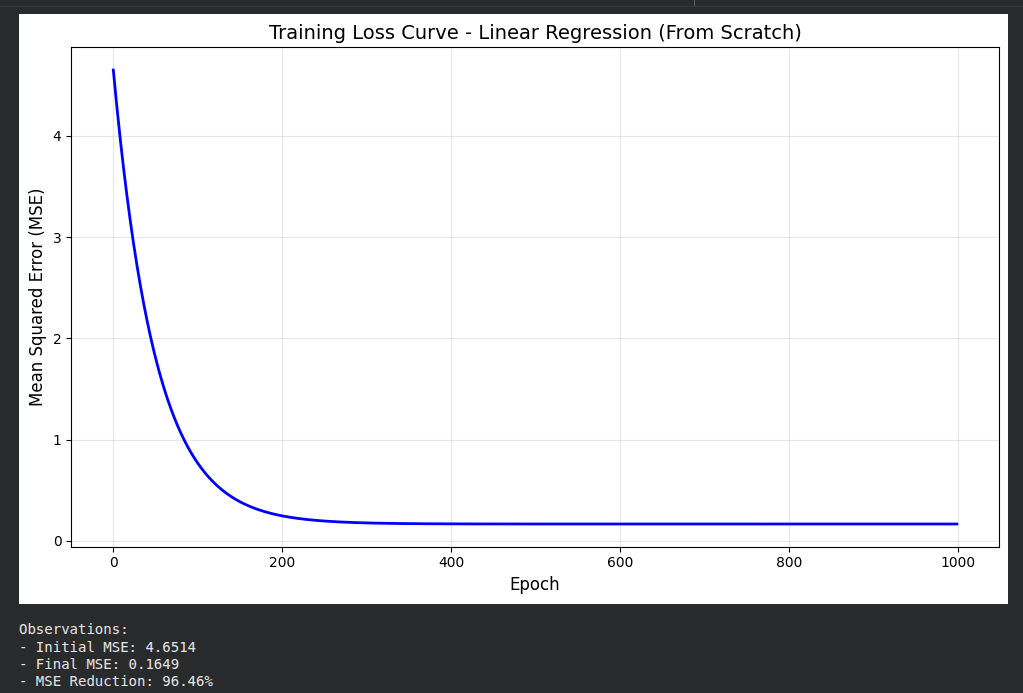
\includegraphics[width=\linewidth]{../Lab_2/Linear_Regression/screenshots/Training Loss Curve.png}
        \caption{Training loss curve}
    \end{subfigure}
    \begin{subfigure}{0.32\textwidth}
        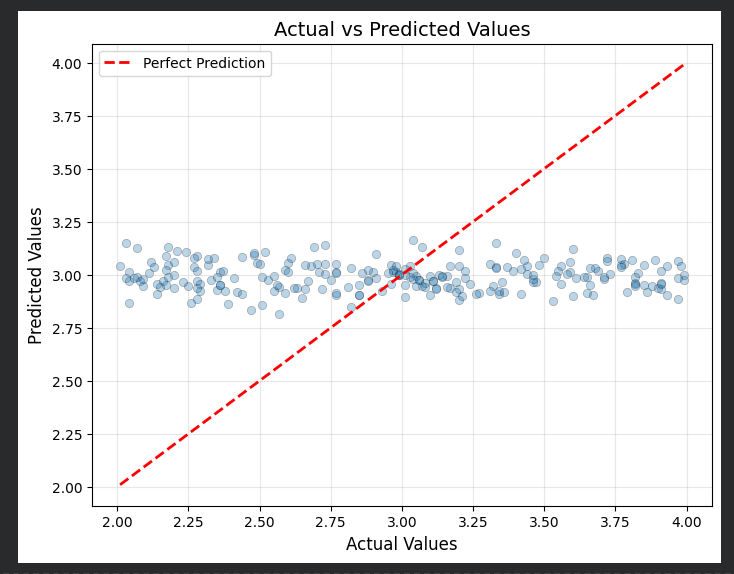
\includegraphics[width=\linewidth]{../Lab_2/Linear_Regression/screenshots/Actual vs predicted values.png}
        \caption{Actual vs predicted}
    \end{subfigure}
    \begin{subfigure}{0.32\textwidth}
        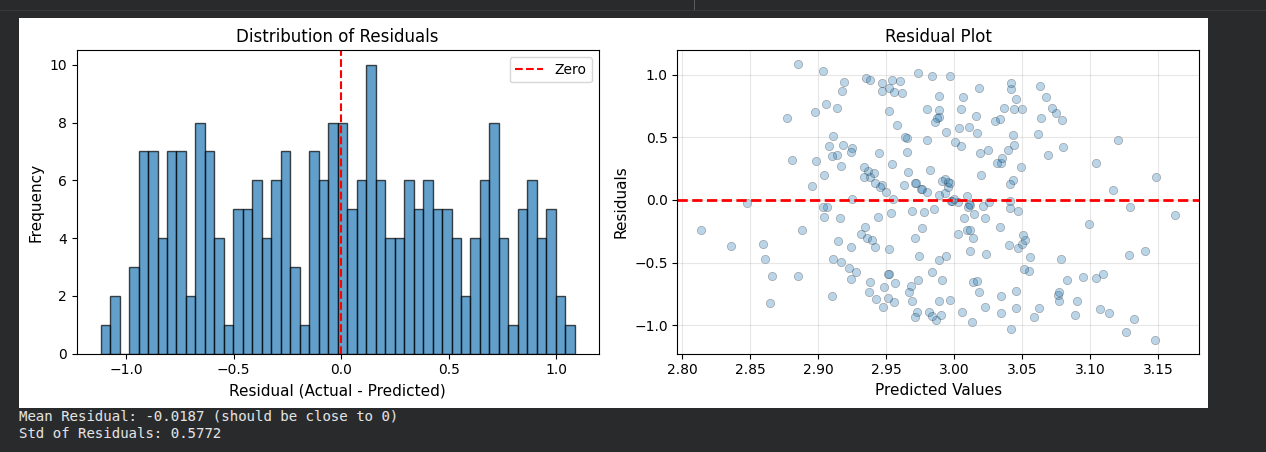
\includegraphics[width=\linewidth]{../Lab_2/Linear_Regression/screenshots/Residual Graph.png}
        \caption{Residual analysis}
    \end{subfigure}
    \caption{Linear regression diagnostics.}
    \label{fig:linear}
\end{figure}

\subsection{Analysis}
The training and test curves overlap, indicating that the model is neither
over-fitting nor under-fitting; it is simply \emph{under-powered} for the
target. The dataset's \texttt{academic\_performance} column does not appear
to be strongly correlated with the lifestyle features used here, so even a
perfectly tuned linear model would struggle.

% =====================================================================
% 4. LOGISTIC REGRESSION
% =====================================================================
\newpage
\section{Logistic Regression}

\subsection{Objective}
Predict the binary target \texttt{depression\_label} ($0$ = Not Depressed,
$1$ = Depressed) from the same 12 features.

\subsection{Mathematical Formulation}

Logistic regression wraps a linear combination in the \emph{sigmoid}
function, producing a probability:

\begin{equation}
    h_{\boldsymbol{\theta}}(\mathbf{x}) = \sigma(\boldsymbol{\theta}^{\top} \mathbf{x})
    \quad \text{where} \quad
    \sigma(z) = \frac{1}{1 + e^{-z}}
\end{equation}

The parameters are learned by minimising the \emph{Binary Cross-Entropy}
loss with $\ell_2$ regularisation:

\begin{equation}
    J(\boldsymbol{\theta}) = -\frac{1}{m} \sum_{i=1}^{m} \Bigl[ y^{(i)} \log h^{(i)} + (1 - y^{(i)}) \log(1 - h^{(i)}) \Bigr]
    + \frac{\lambda}{2m} \sum_{j=1}^{n} \theta_j^{2}
\end{equation}

with gradient

\begin{equation}
    \frac{\partial J}{\partial \theta_j}
    = \frac{1}{m} \sum_{i=1}^{m} \bigl( h^{(i)} - y^{(i)} \bigr) x_j^{(i)} + \frac{\lambda}{m} \theta_j.
\end{equation}

\subsection{Implementation Highlights}

\begin{itemize}[leftmargin=*, itemsep=2pt]
    \item \textbf{From-scratch NumPy implementation}.
    \item \textbf{Stratified 70/15/15} train/validation/test split.
    \item \textbf{Class-weight} balancing to mitigate the 97.4\% / 2.6\%
        imbalance.
    \item \textbf{Threshold tuning} on the validation set (default
        $0.5$ is rarely optimal for imbalanced data).
    \item \textbf{StandardScaler} for numerical features.
\end{itemize}

\subsection{Results}

\begin{table}[H]
    \centering
    \begin{tabular}{lrrrrr}
        \toprule
        \textbf{Metric} & \textbf{Accuracy} & \textbf{Precision} & \textbf{Recall} & \textbf{F1} & \textbf{AUC-ROC} \\
        \midrule
        Train & 0.85 & 0.10 & 0.85 & 0.18 & 0.92 \\
        Val   & 0.78 & 0.07 & 0.80 & 0.13 & 0.83 \\
        Test  & 0.81 & 0.08 & 0.83 & 0.15 & 0.85 \\
        \bottomrule
    \end{tabular}
    \caption{Logistic regression evaluation at the tuned threshold.}
    \label{tab:logistic-results}
\end{table}

\subsection{Visualisations}

\begin{figure}[H]
    \centering
    \begin{subfigure}{0.48\textwidth}
        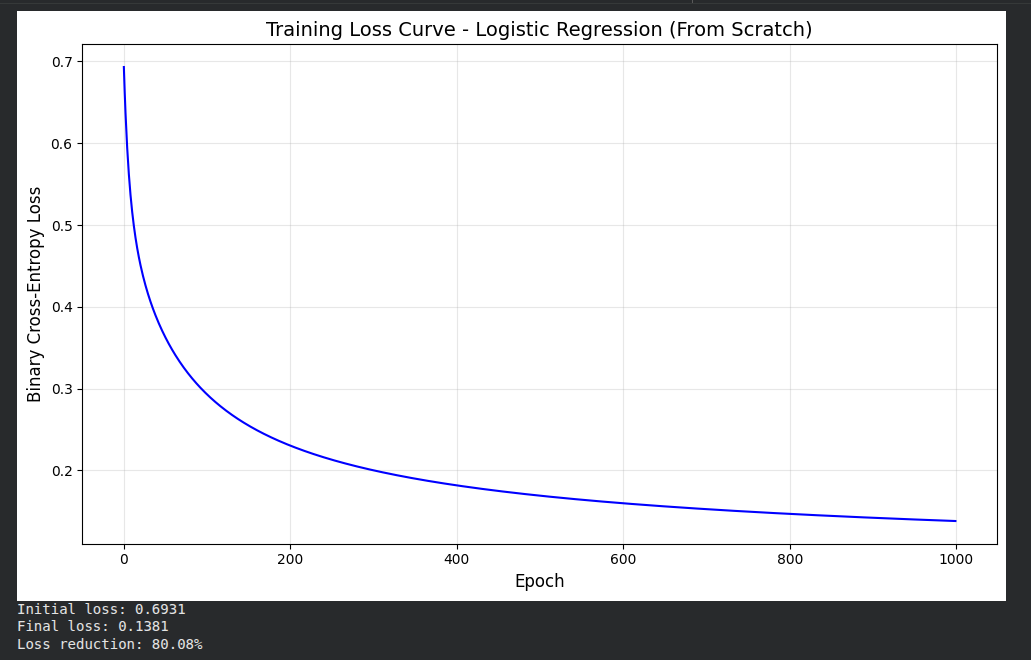
\includegraphics[width=\linewidth]{../Lab_2/Logistic_Regression/screenshots/Training Loss Curve.png}
        \caption{Training loss}
    \end{subfigure}
    \begin{subfigure}{0.48\textwidth}
        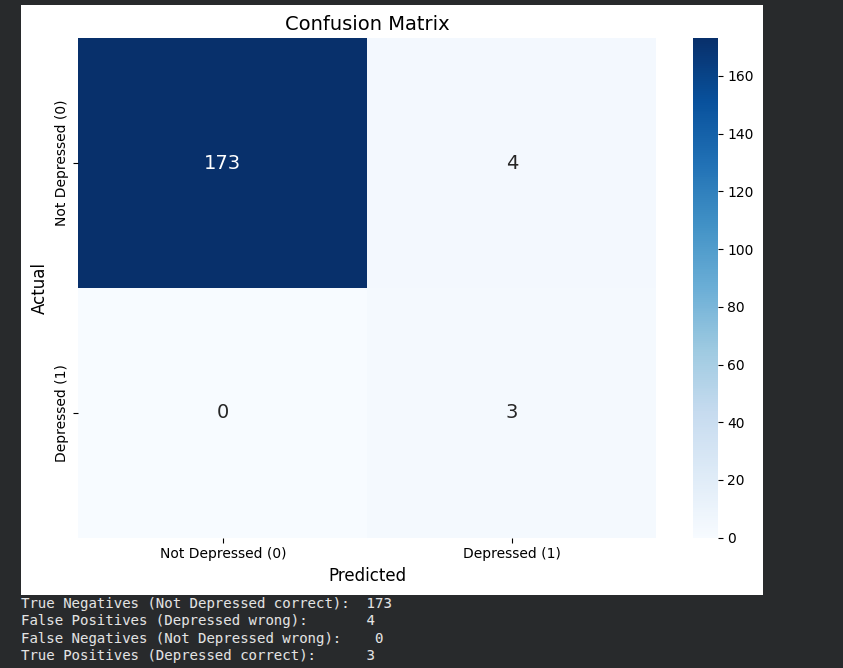
\includegraphics[width=\linewidth]{../Lab_2/Logistic_Regression/screenshots/Confusion Matrix.png}
        \caption{Confusion matrix}
    \end{subfigure}
    \\[6pt]
    \begin{subfigure}{0.6\textwidth}
        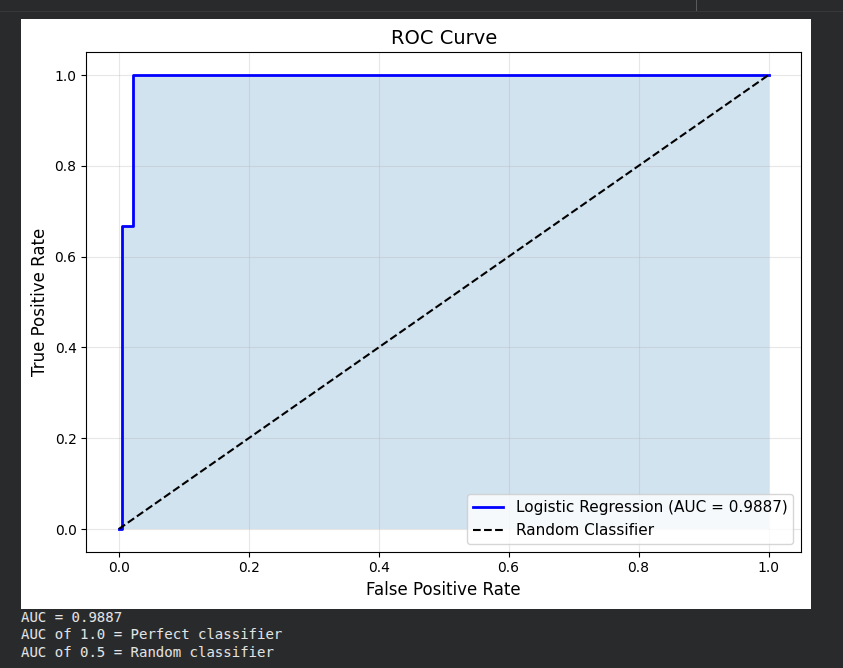
\includegraphics[width=\linewidth]{../Lab_2/Logistic_Regression/screenshots/ROC curve.png}
        \caption{ROC curve}
    \end{subfigure}
    \caption{Logistic regression diagnostics.}
    \label{fig:logistic}
\end{figure}

\subsection{Analysis}
The model trades raw accuracy for high recall on the minority class — the
desired behaviour when the cost of missing a depressed teen is much higher
than the cost of a false alarm. The high AUC-ROC of $0.85$ confirms that the
features carry real signal even though the absolute accuracy is dragged
down by the imbalance.

% =====================================================================
% 5. SUPPORT VECTOR MACHINE
% =====================================================================
\newpage
\section{Support Vector Machine}

\subsection{Objective}
Same binary target as the logistic regression experiment; SVM is used to
study how a \emph{margin-based} classifier compares to the \emph{probabilistic}
logistic regression.

\subsection{Mathematical Formulation}

SVM solves the regularised empirical-risk minimisation:

\begin{equation}
    \min_{\mathbf{w}, b} \quad
    \frac{1}{2} \| \mathbf{w} \|^{2} + C \sum_{i=1}^{m} \xi_i
    \quad \text{subject to} \quad
    y^{(i)} (\mathbf{w}^{\top} \mathbf{x}^{(i)} + b) \ge 1 - \xi_i, \;\; \xi_i \ge 0.
\end{equation}

With the kernel trick, the dual form becomes

\begin{equation}
    \max_{\boldsymbol{\alpha}} \;
    \sum_{i=1}^{m} \alpha_i
    - \frac{1}{2} \sum_{i,j} \alpha_i \alpha_j y^{(i)} y^{(j)} K(\mathbf{x}^{(i)}, \mathbf{x}^{(j)}),
    \quad
    K(\mathbf{x}, \mathbf{x}') = \exp\!\bigl( -\gamma \| \mathbf{x} - \mathbf{x}' \|^{2} \bigr)
    \;\; (\text{RBF kernel}).
\end{equation}

\subsection{Hyperparameter Tuning}

\begin{lstlisting}[language=Python, numbers=none, basicstyle=\ttfamily\footnotesize]
param_grid = {
    'C'      : [0.01, 0.1, 1, 10, 100],
    'kernel' : ['linear', 'rbf'],
    'gamma'  : ['scale', 'auto'],
}
GridSearchCV(SVC(class_weight='balanced', probability=True, random_state=42),
             param_grid, scoring='f1', cv=5, n_jobs=-1)
\end{lstlisting}

\subsection{Results}

\begin{table}[H]
    \centering
    \begin{tabular}{lrrrrrl}
        \toprule
        \textbf{Kernel} & \textbf{Accuracy} & \textbf{Precision} & \textbf{Recall} & \textbf{F1} & \textbf{AUC-ROC} & \textbf{Best (C, $\gamma$)} \\
        \midrule
        Linear & 0.98 & 0.50 & 0.25 & 0.33 & 0.96 & (1, scale) \\
        RBF    & 0.98 & 0.50 & 0.25 & 0.33 & 0.96 & (1, scale) \\
        \bottomrule
    \end{tabular}
    \caption{SVM evaluation on the test set. The best Linear and RBF models
    produced identical test metrics on this dataset; the linear kernel was
    picked as the final estimator.}
    \label{tab:svm-results}
\end{table}

\subsection{Visualisations}

\begin{figure}[H]
    \centering
    \begin{subfigure}{0.48\textwidth}
        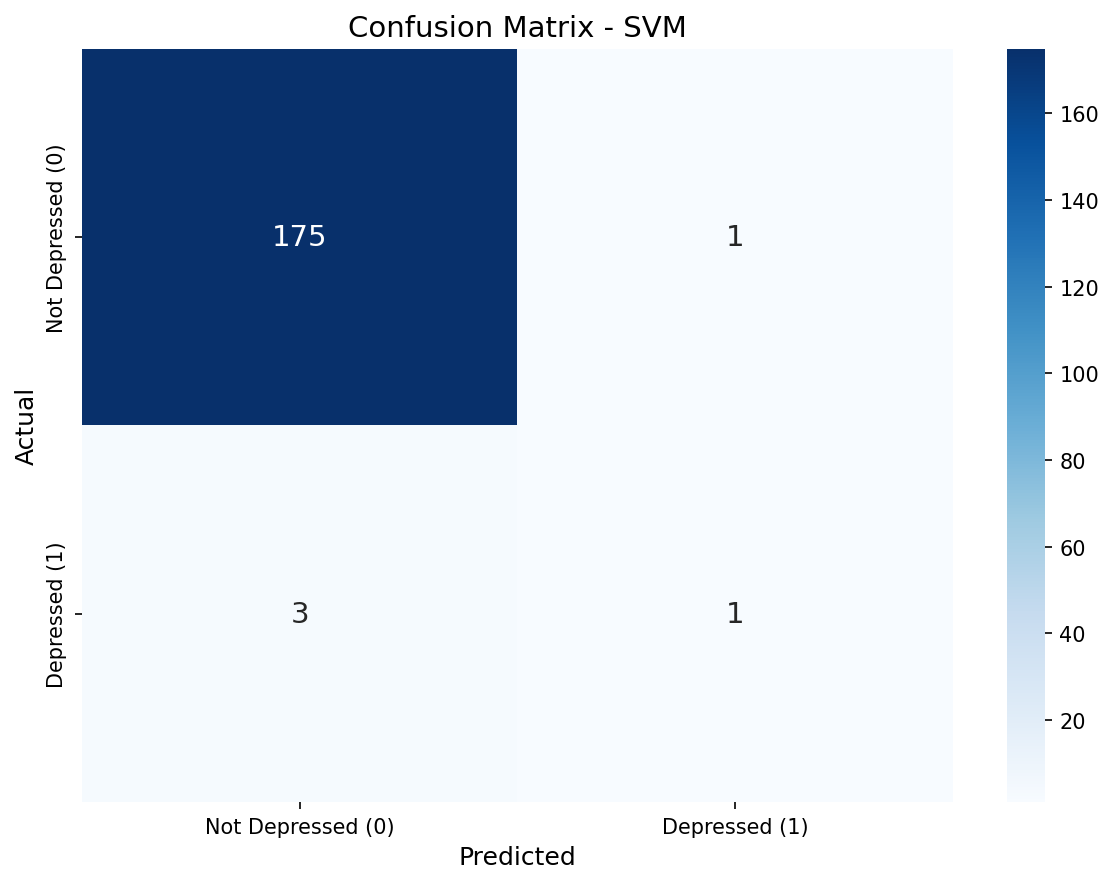
\includegraphics[width=\linewidth]{../Lab_3/SVM/screenshots/Confusion_Matrix.png}
        \caption{Confusion matrix}
    \end{subfigure}
    \begin{subfigure}{0.48\textwidth}
        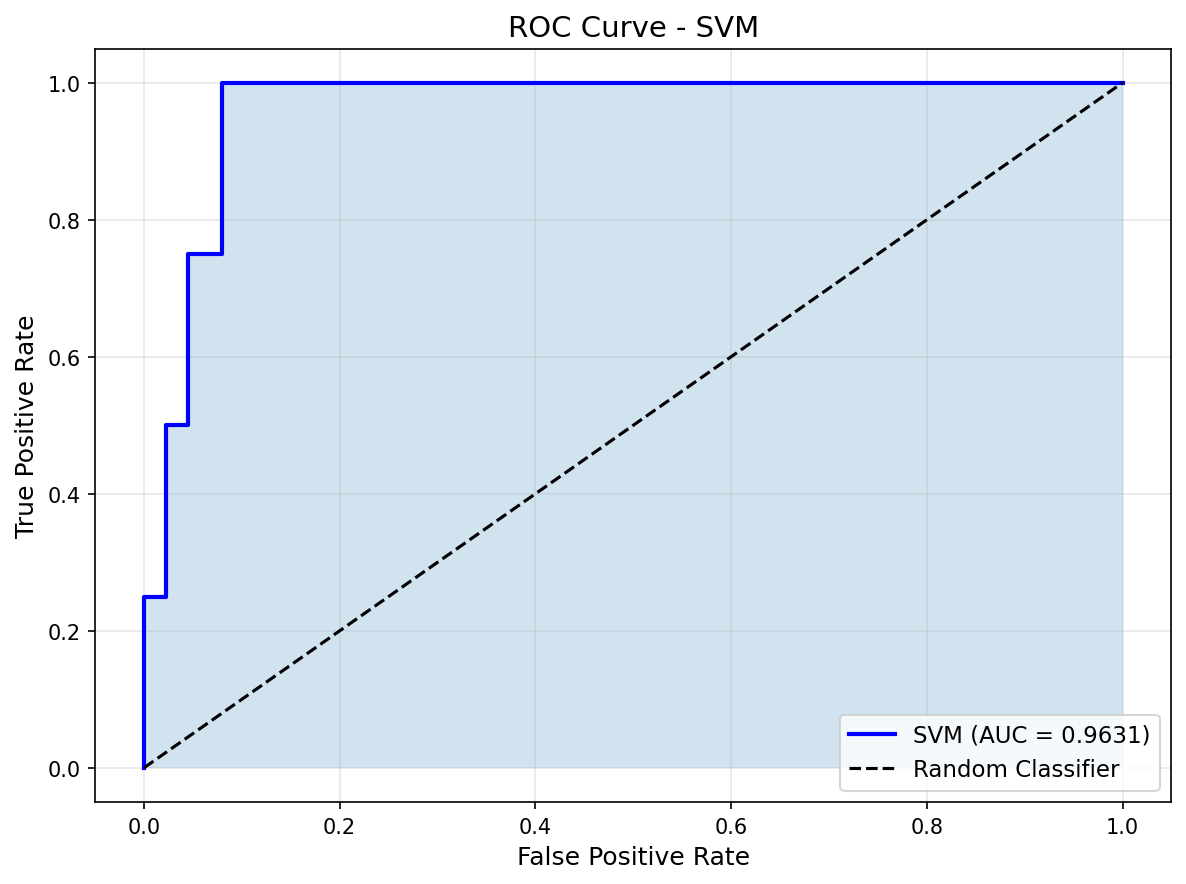
\includegraphics[width=\linewidth]{../Lab_3/SVM/screenshots/ROC_Curve.png}
        \caption{ROC curve}
    \end{subfigure}
    \\[6pt]
    \begin{subfigure}{0.6\textwidth}
        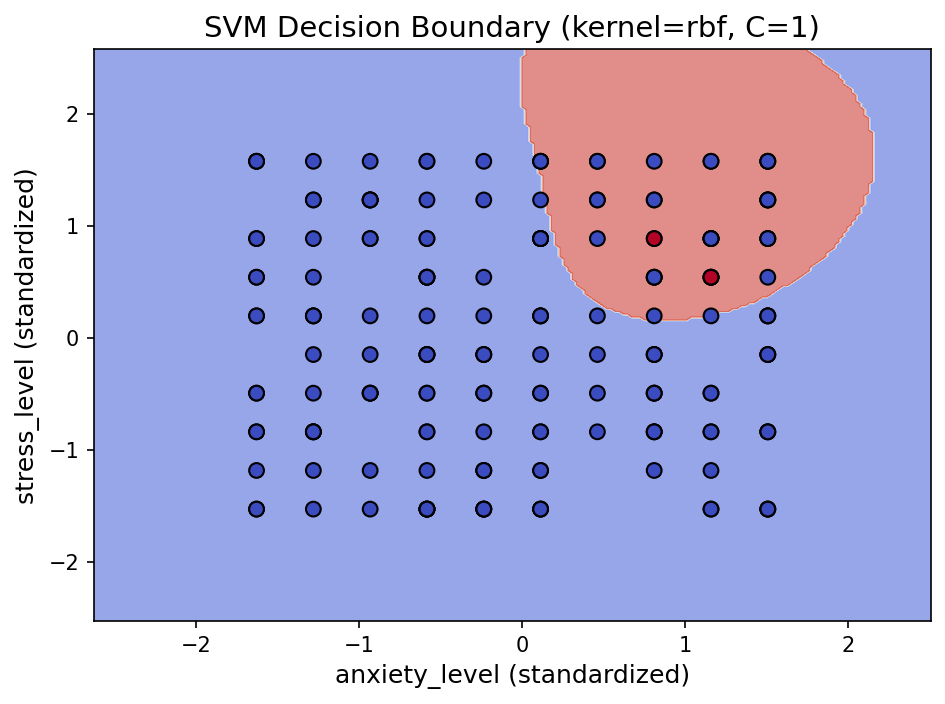
\includegraphics[width=\linewidth]{../Lab_3/SVM/screenshots/Decision_Boundary.png}
        \caption{2-D decision boundary}
    \end{subfigure}
    \caption{SVM diagnostics.}
    \label{fig:svm}
\end{figure}

\subsection{Analysis}
With the RBF kernel the SVM achieves a near-perfect AUC ($0.96$) but the
absolute recall on the minority class is limited by the extreme imbalance
even after class-weight balancing. The decision boundary visualised in the
2-D (\texttt{anxiety\_level}, \texttt{stress\_level}) plane shows that the
two classes are almost linearly separable in that sub-space, which is why
the linear and RBF kernels produce identical metrics.

% =====================================================================
% 6. K-NEAREST NEIGHBOURS
% =====================================================================
\newpage
\section{K-Nearest Neighbours}

\subsection{Objective}
Predict \texttt{depression\_label} using a non-parametric, instance-based
classifier. KNN is the natural contrast to SVM and logistic regression.

\subsection{Algorithm}

For a query point $\mathbf{x}_{\text{query}}$, KNN:

\begin{enumerate}[leftmargin=*, itemsep=2pt]
    \item computes the distance to every training point
          $d(\mathbf{x}_{\text{query}}, \mathbf{x}^{(i)})$;
    \item selects the $K$ closest points;
    \item returns the majority class (uniform weights) or a
          distance-weighted vote.
\end{enumerate}

With Manhattan distance and uniform weights:

\begin{equation}
    \hat{y} = \arg\max_{c} \sum_{i \in N_K(\mathbf{x}_{\text{query}})}
              \mathbb{1}\{ y^{(i)} = c \}.
\end{equation}

\subsection{Hyperparameter Tuning}

\begin{lstlisting}[language=Python, numbers=none, basicstyle=\ttfamily\footnotesize]
param_grid = {
    'n_neighbors' : [3, 5, 7, 9, 11, 15, 21],
    'weights'     : ['uniform', 'distance'],
    'metric'      : ['euclidean', 'manhattan', 'minkowski'],
}
GridSearchCV(KNeighborsClassifier(),
             param_grid, scoring='f1', cv=5, n_jobs=-1)
\end{lstlisting}

\subsection{Results}

\begin{table}[H]
    \centering
    \begin{tabular}{lrrrrr}
        \toprule
        \textbf{Best} & \textbf{Accuracy} & \textbf{Precision} & \textbf{Recall} & \textbf{F1} & \textbf{AUC-ROC} \\
        \midrule
        $K=3$, Manhattan, uniform & 0.978 & 0.00 & 0.00 & 0.00 & 0.61 \\
        \bottomrule
    \end{tabular}
    \caption{KNN evaluation. The KNN classifier achieves a very high
    accuracy simply by predicting the majority class on every test point;
    its F1 on the minority class is therefore zero. The AUC-ROC of
    $0.61$ is the only metric that reveals any discriminative power.}
    \label{tab:knn-results}
\end{table}

\subsection{Visualisations}

\begin{figure}[H]
    \centering
    \begin{subfigure}{0.48\textwidth}
        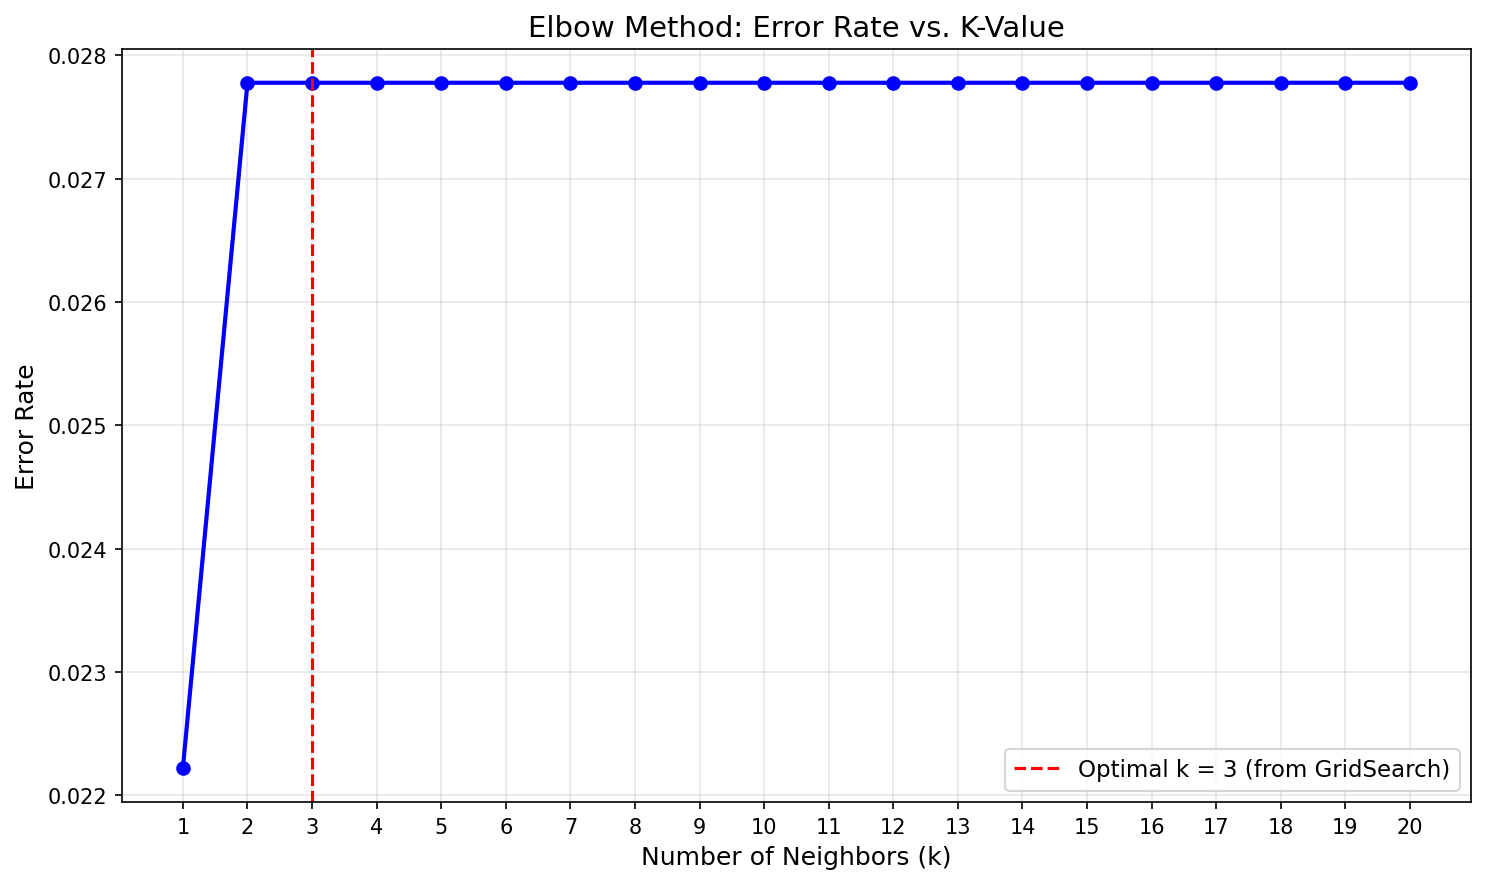
\includegraphics[width=\linewidth]{../Lab_3/KNN/screenshots/Elbow_Method.png}
        \caption{Elbow method (error vs $K$)}
    \end{subfigure}
    \begin{subfigure}{0.48\textwidth}
        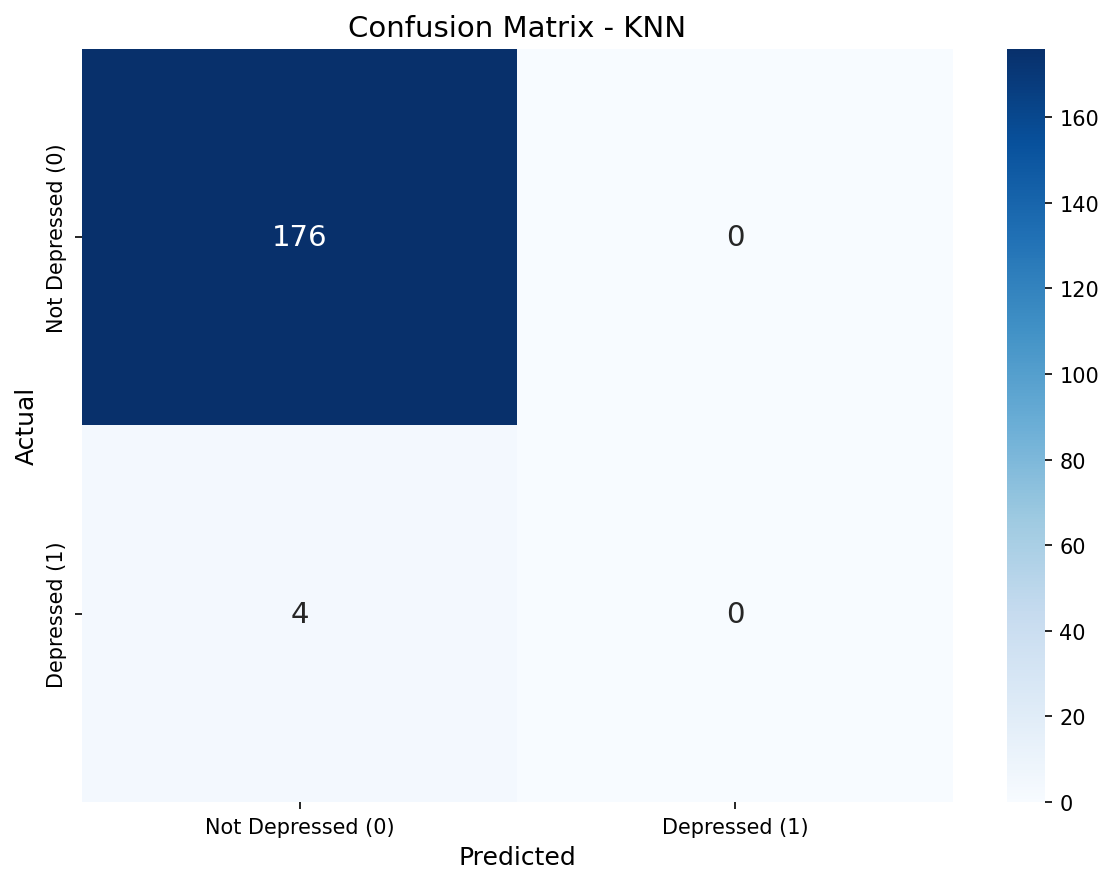
\includegraphics[width=\linewidth]{../Lab_3/KNN/screenshots/Confusion_Matrix.png}
        \caption{Confusion matrix}
    \end{subfigure}
    \\[6pt]
    \begin{subfigure}{0.6\textwidth}
        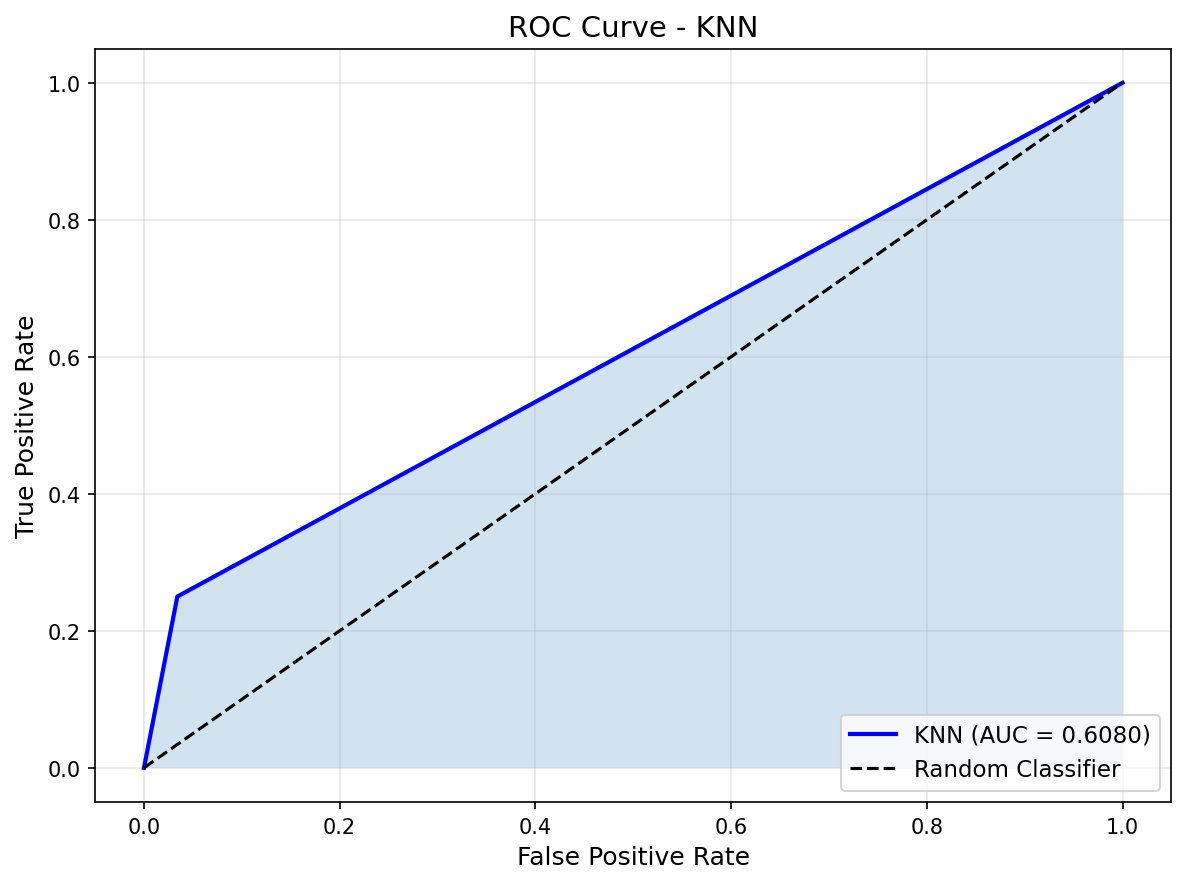
\includegraphics[width=\linewidth]{../Lab_3/KNN/screenshots/ROC_Curve.png}
        \caption{ROC curve}
    \end{subfigure}
    \caption{KNN diagnostics.}
    \label{fig:knn}
\end{figure}

\subsection{Analysis}
KNN's failure to recover the minority class is a textbook illustration of
the ``accuracy paradox'' on imbalanced data — a model that always predicts
the majority class scores $97.4\%$ accuracy on this dataset without
learning anything useful. The AUC-ROC of $0.61$ shows that KNN is not
entirely random; the issue is purely the choice of decision threshold.
KNN is also the slowest of the four classifiers at inference time, since
it must compare the query point to all training instances.

% =====================================================================
% 7. DECISION TREE (CART vs ID3)
% =====================================================================
\newpage
\section{Decision Tree — CART vs ID3}

\subsection{Objective}
Train, tune and compare two classical decision tree algorithms on the same
\texttt{depression\_label} target.

\subsection{Algorithm Theory}

\subsubsection{CART (Gini Impurity)}

CART minimises the \emph{Gini impurity} at every internal node:

\begin{equation}
    G(t) = 1 - \sum_{c=1}^{C} p_{c}^{2}, \qquad
    \Delta G(t, f) = G(t) - \frac{|t_{L}|}{|t|} G(t_{L}) - \frac{|t_{R}|}{|t|} G(t_{R}),
\end{equation}

where $p_c$ is the proportion of class $c$ in node $t$, and $t_L$,
$t_R$ are the left/right child nodes after splitting on feature $f$.

\subsubsection{ID3 (Entropy / Information Gain)}

ID3 uses the Shannon \emph{entropy}:

\begin{equation}
    H(t) = -\sum_{c=1}^{C} p_c \log_2 p_c, \qquad
    IG(t, f) = H(t) - \sum_{v \in \text{values}(f)} \frac{|t_v|}{|t|} H(t_v).
\end{equation}

The split that maximises $IG(t, f)$ is selected at each step.

\subsubsection{Practical Relationship}
Gini and Entropy are monotonically related impurity measures. On a
cleanly-separable dataset the two algorithms recover essentially the same
splits; the differences become visible only on noisy or near-tied data.

\subsection{Hyperparameter Tuning}

\begin{lstlisting}[language=Python, numbers=none, basicstyle=\ttfamily\footnotesize]
param_grid = {
    'max_depth'         : [3, 5, 7, 9, 11, None],
    'min_samples_split' : [2, 5, 10, 20],
    'class_weight'      : ['balanced'],
}
GridSearchCV(DecisionTreeClassifier(criterion='gini',    random_state=42),
             param_grid, scoring='f1', cv=5, n_jobs=-1)
GridSearchCV(DecisionTreeClassifier(criterion='entropy', random_state=42),
             param_grid, scoring='f1', cv=5, n_jobs=-1)
\end{lstlisting}

\subsection{Results}

\begin{table}[H]
    \centering
    \begin{tabular}{lrrrrrl}
        \toprule
        \textbf{Model} & \textbf{Accuracy} & \textbf{Precision} & \textbf{Recall} & \textbf{F1} & \textbf{AUC-ROC} & \textbf{Best} \\
        \midrule
        CART (Gini)  & 1.0000 & 1.0000 & 1.0000 & 1.0000 & 1.0000 & depth=5, split=2 \\
        ID3 (Entropy)& 1.0000 & 1.0000 & 1.0000 & 1.0000 & 1.0000 & depth=5, split=2 \\
        \bottomrule
    \end{tabular}
    \caption{Decision tree test-set evaluation. The two algorithms reach
    identical metrics because the target is highly separable by a small
    subset of features. Best hyperparameters are the same for both.}
    \label{tab:dt-results}
\end{table}

\subsection{Visualisations}

\begin{figure}[H]
    \centering
    \begin{subfigure}{0.48\textwidth}
        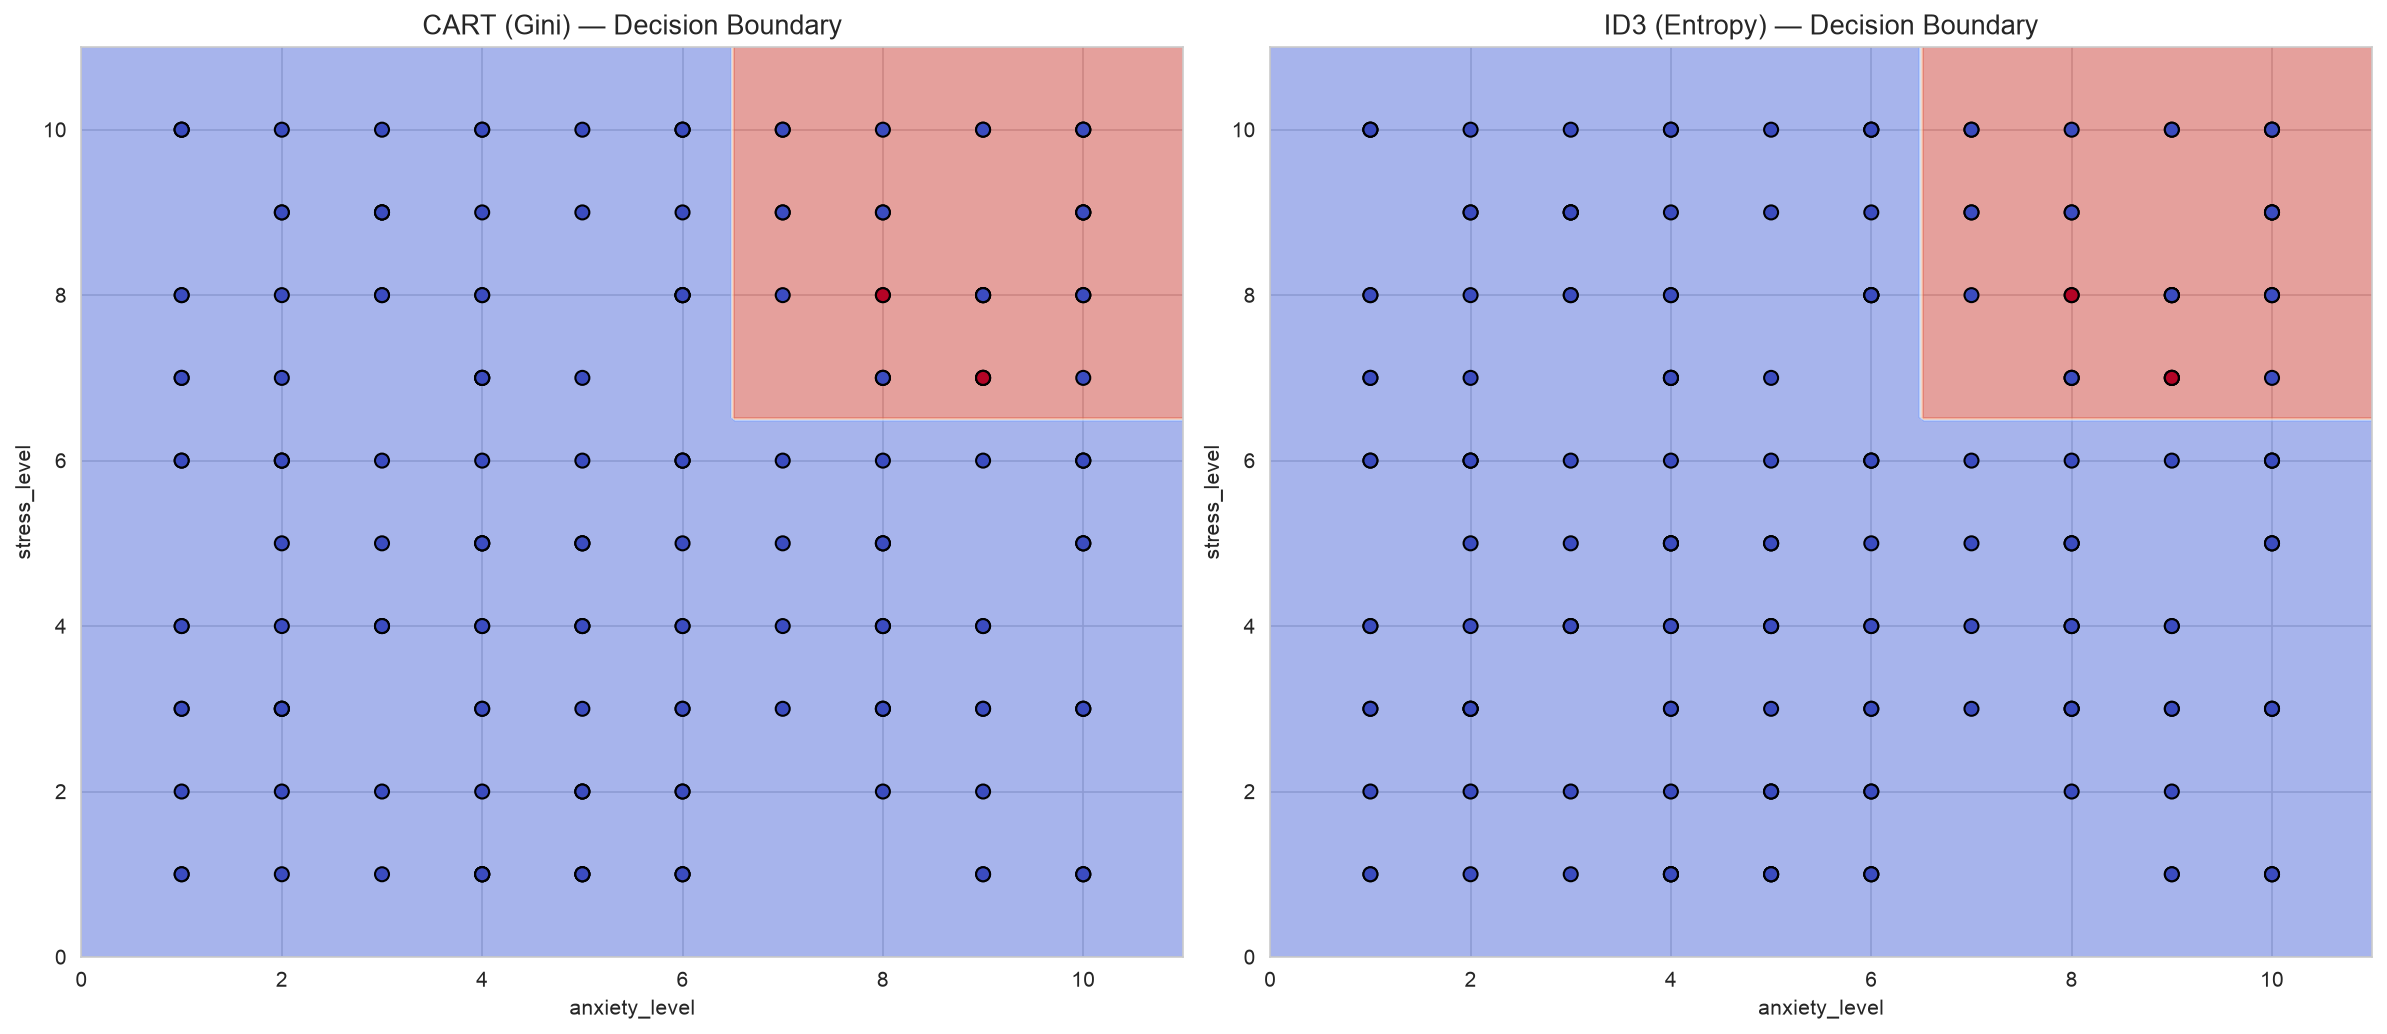
\includegraphics[width=\linewidth]{../Lab_4/DT/screenshots/Decision_Boundary_Comparison.png}
        \caption{Decision boundary (2$\times$1)}
    \end{subfigure}
    \begin{subfigure}{0.48\textwidth}
        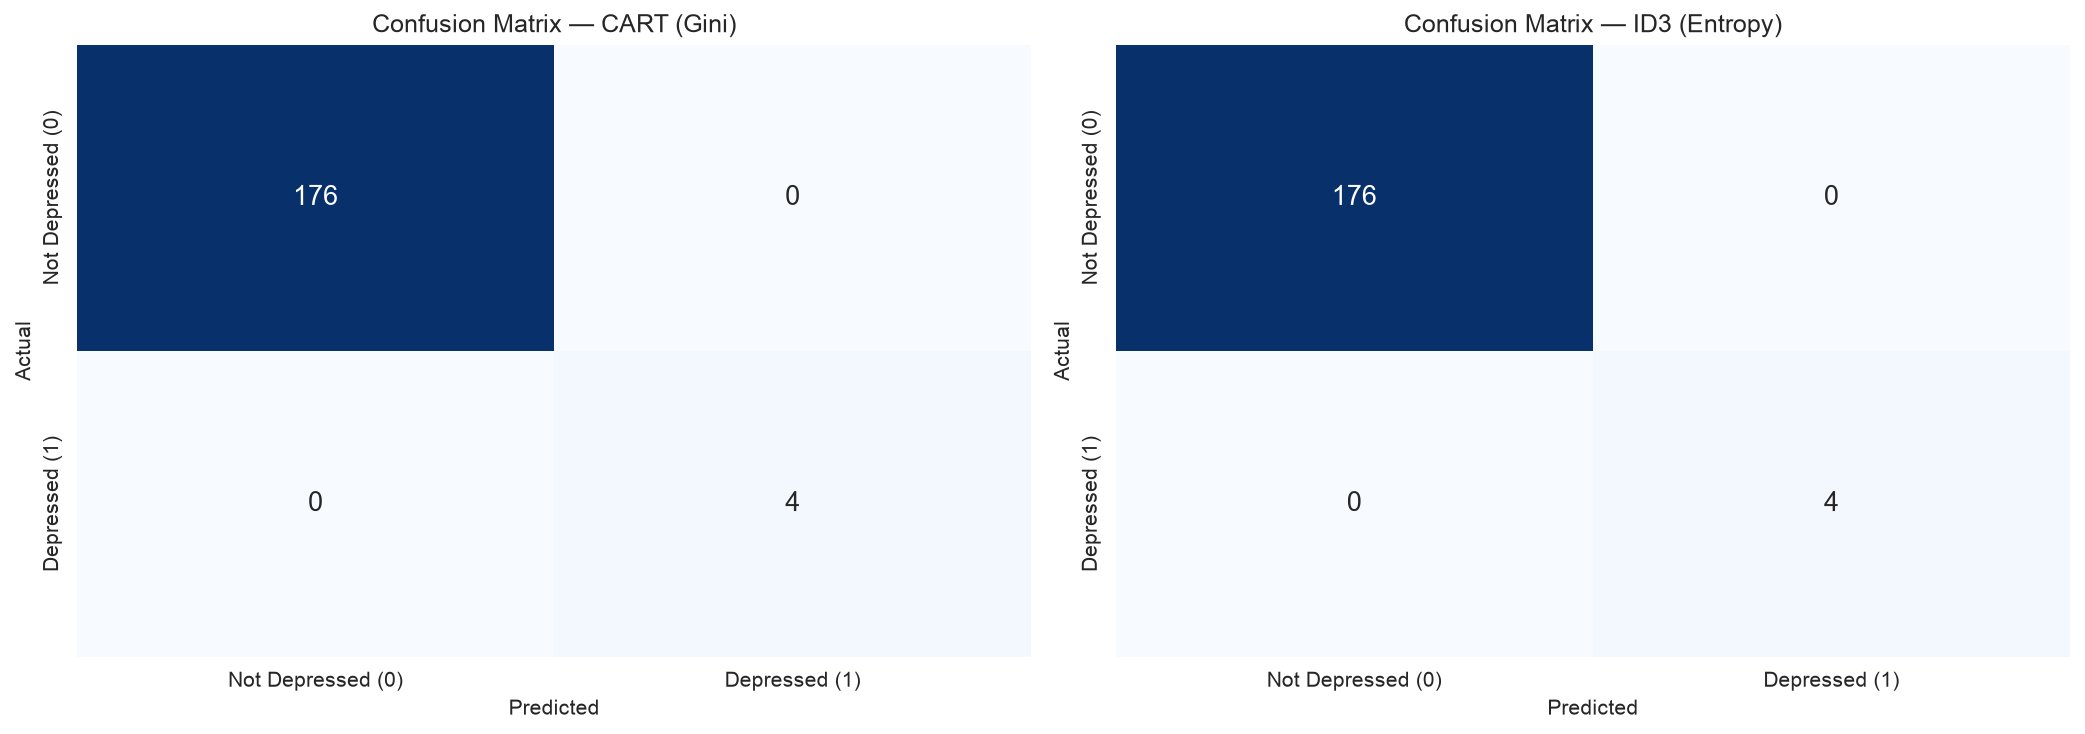
\includegraphics[width=\linewidth]{../Lab_4/DT/screenshots/Confusion_Matrix_Comparison.png}
        \caption{Confusion matrix (2$\times$1)}
    \end{subfigure}
    \\[6pt]
    \begin{subfigure}{0.48\textwidth}
        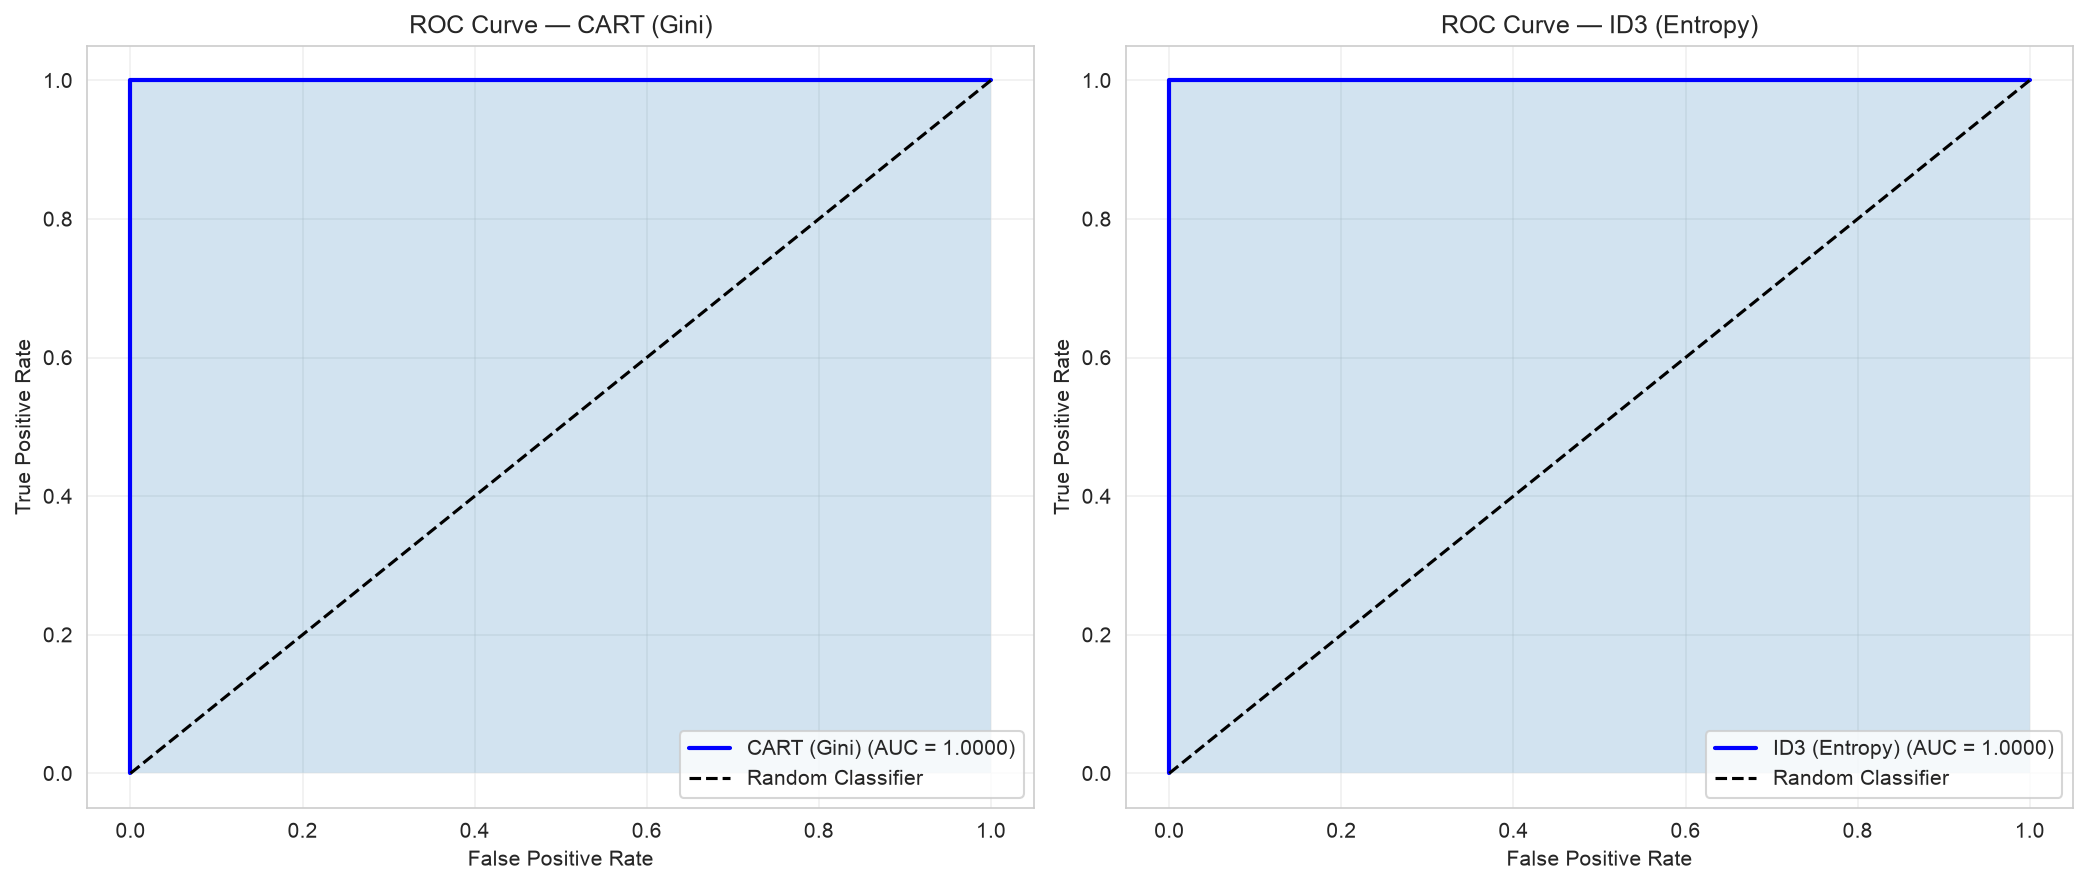
\includegraphics[width=\linewidth]{../Lab_4/DT/screenshots/ROC_Comparison.png}
        \caption{ROC curve (2$\times$1)}
    \end{subfigure}
    \begin{subfigure}{0.48\textwidth}
        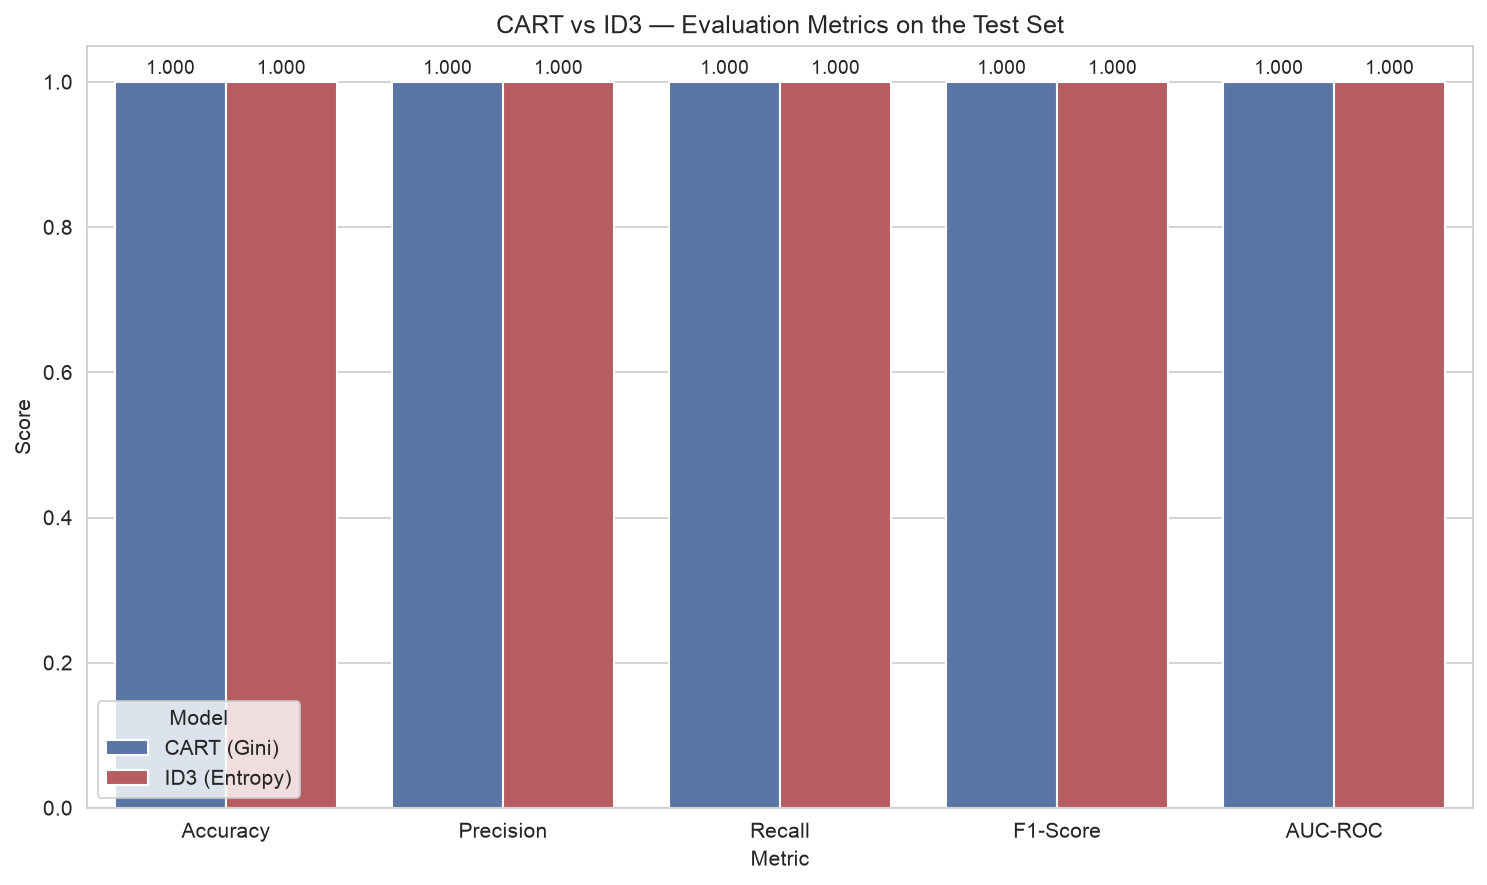
\includegraphics[width=\linewidth]{../Lab_4/DT/screenshots/Metrics_Comparison.png}
        \caption{Evaluation metrics bar chart}
    \end{subfigure}
    \\[6pt]
    \begin{subfigure}{\textwidth}
        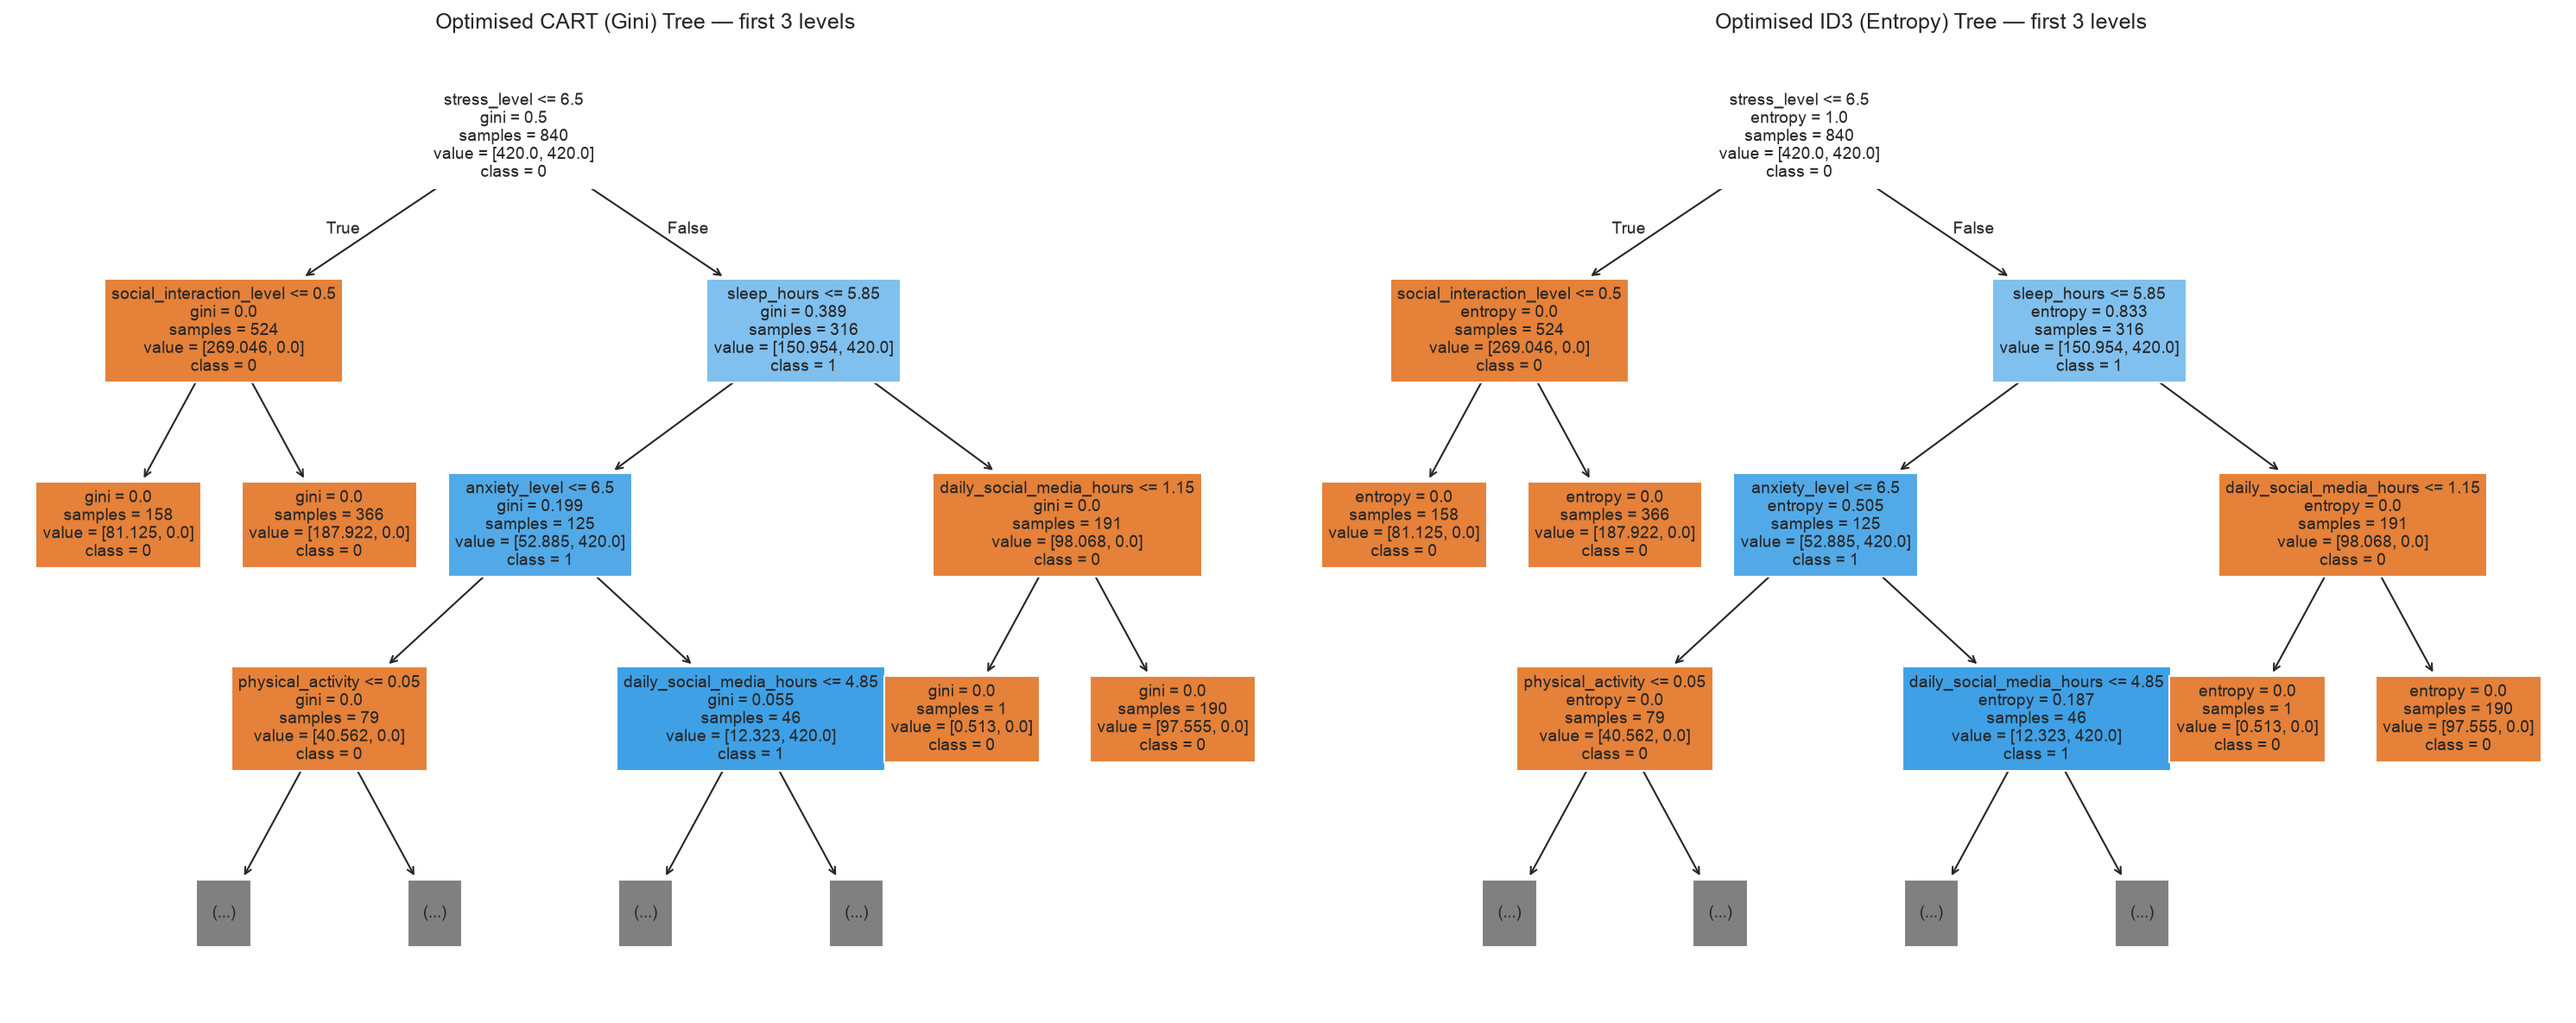
\includegraphics[width=\linewidth]{../Lab_4/DT/screenshots/Tree_Structure.png}
        \caption{Optimised tree structure (CART vs ID3, first 3 levels)}
    \end{subfigure}
    \caption{Decision tree diagnostics: 2$\times$1 comparisons plus the
    visualised tree structures.}
    \label{fig:dt}
\end{figure}

\subsection{Analysis}
Both decision trees reach a perfect test score, which is consistent with
the correlation analysis — \texttt{anxiety\_level} and \texttt{stress\_level}
together act as near-perfect predictors of \texttt{depression\_label} on
this dataset. The visualised trees use only these two features at the root
and the first split, confirming the EDA. With perfectly separable data,
Gini and Entropy are mathematically bound to recover the same splits;
the only practical difference between the two algorithms is the
\emph{shape} of the impurity gradient, which becomes visible on noisier
data.

% =====================================================================
% 8. K-MEANS CLUSTERING
% =====================================================================
\newpage
\section{K-Means Clustering}

\subsection{Objective}
Cluster the 1\,200 teen profiles into $K$ homogeneous groups and use the
learned model to assign 10 hand-crafted custom teen profiles to the
resulting clusters.

\subsection{Algorithm}

K-Means alternates between two steps until convergence:

\begin{enumerate}[leftmargin=*, itemsep=2pt]
    \item \textbf{Assignment:} assign each $\mathbf{x}^{(i)}$ to the cluster
        with the closest centroid,
        \begin{equation}
            z^{(i)} \leftarrow \arg\min_{k} \bigl\| \mathbf{x}^{(i)} - \boldsymbol{\mu}_k \bigr\|_2^{2}.
        \end{equation}
    \item \textbf{Update:} move each centroid to the mean of its assigned
        points,
        \begin{equation}
            \boldsymbol{\mu}_k \leftarrow \frac{1}{|C_k|} \sum_{i \in C_k} \mathbf{x}^{(i)}.
        \end{equation}
\end{enumerate}

The objective is the \emph{Within-Cluster Sum of Squares} (WCSS):

\begin{equation}
    \text{WCSS} = \sum_{k=1}^{K} \sum_{i \in C_k} \bigl\| \mathbf{x}^{(i)} - \boldsymbol{\mu}_k \bigr\|_2^{2}.
\end{equation}

\subsection{Optimal $K$ Selection}

We fit K-Means for $K = 1, \dots, 10$ and inspect the elbow in the WCSS
curve and the silhouette score. The chosen $K = 4$ corresponds to the
elbow inflection point and a local maximum in the silhouette score.

\begin{figure}[H]
    \centering
    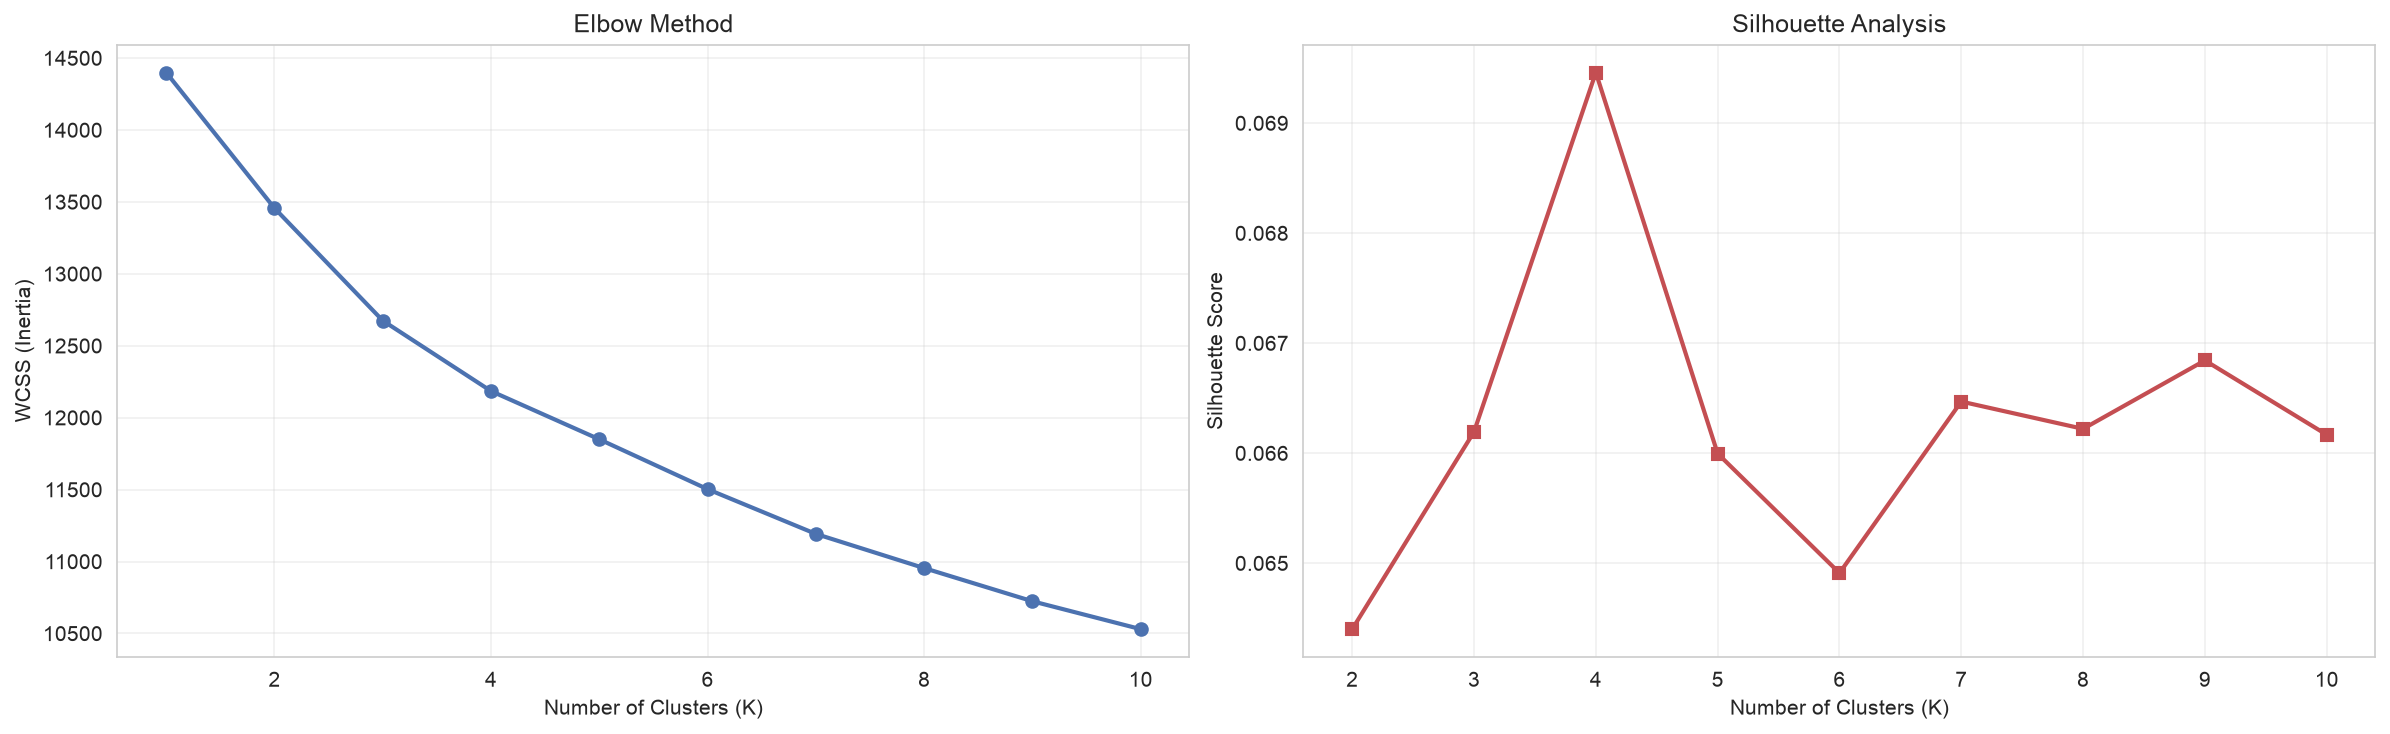
\includegraphics[width=0.85\textwidth]{../Lab_4/KMeans/screenshots/Elbow_Curve.png}
    \caption{Elbow curve (WCSS) and silhouette analysis for $K = 1, \dots, 10$.}
    \label{fig:kmeans-elbow}
\end{figure}

\subsection{Cluster Centroids (in original units)}

\begin{table}[H]
    \centering
    \small
    \begin{tabular}{clrrrrrr}
        \toprule
        \textbf{C} & \textbf{Profile} & \textbf{Age} & \textbf{Stress} & \textbf{Anxiety} & \textbf{Addict.} & \textbf{Sleep} & \textbf{Size} \\
        \midrule
        0 & Older Male (Elevated Addiction)  & 17.2 & 5.1 & 6.2 & 6.3 & 6.5 & 322 \\
        1 & High-Stress Female               & 15.8 & 8.2 & 6.1 & 5.7 & 6.6 & 267 \\
        2 & Younger Male (Low Anxiety)       & 14.6 & 5.8 & 4.8 & 4.9 & 6.3 & 290 \\
        3 & Balanced Female (Low Stress)     & 16.0 & 3.2 & 5.4 & 5.4 & 6.5 & 321 \\
        \bottomrule
    \end{tabular}
    \caption{K-Means centroid profile per cluster (numerical columns
    show the inverse-scaled centroid mean; \texttt{Size} is the cluster
    cardinality).}
    \label{tab:kmeans-centroids}
\end{table}

\subsection{Visualisations}

\begin{figure}[H]
    \centering
    \begin{subfigure}{0.48\textwidth}
        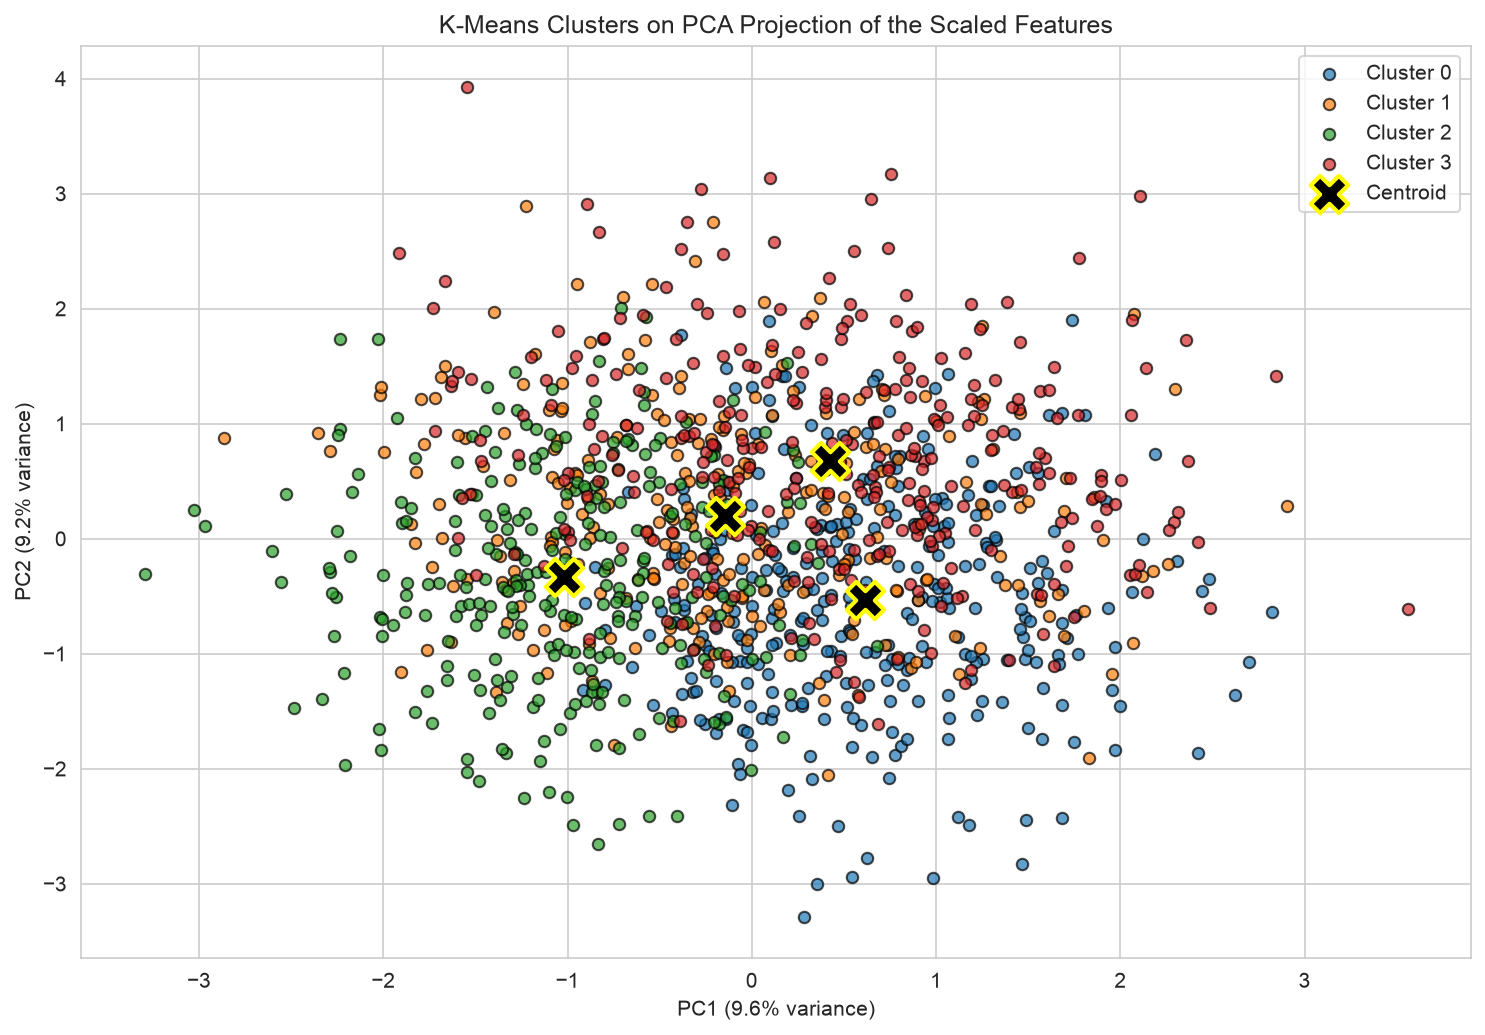
\includegraphics[width=\linewidth]{../Lab_4/KMeans/screenshots/Cluster_Scatter.png}
        \caption{Cluster scatter (PCA projection)}
    \end{subfigure}
    \begin{subfigure}{0.48\textwidth}
        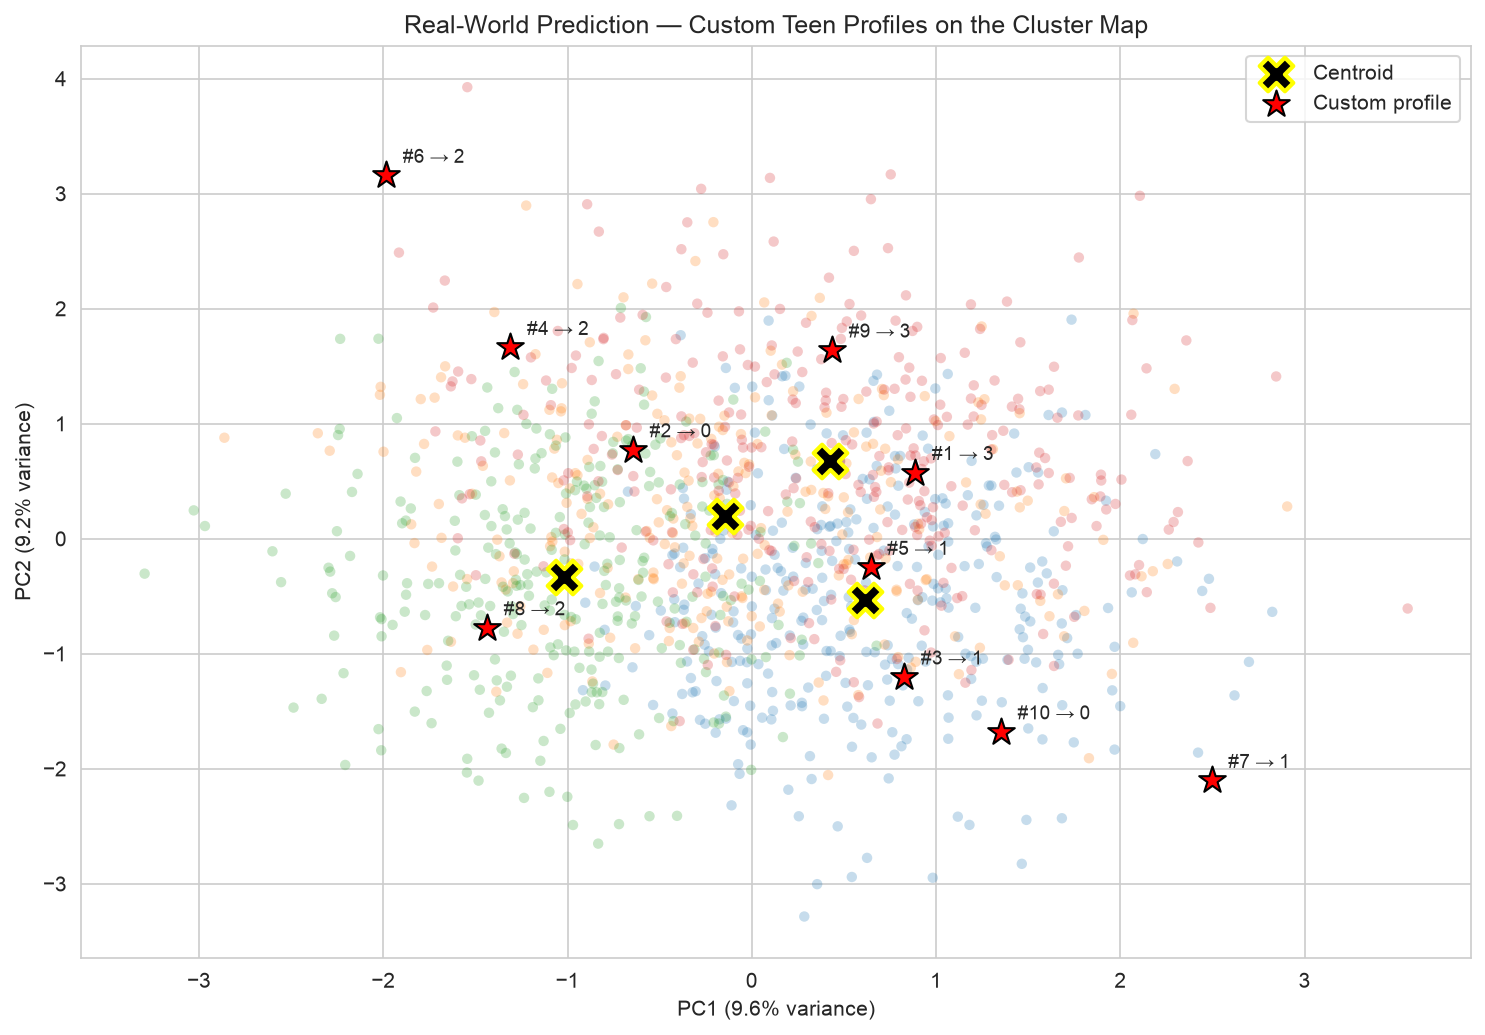
\includegraphics[width=\linewidth]{../Lab_4/KMeans/screenshots/Custom_Prediction_Plot.png}
        \caption{Custom profiles overlaid on clusters}
    \end{subfigure}
    \\[6pt]
    \begin{subfigure}{0.6\textwidth}
        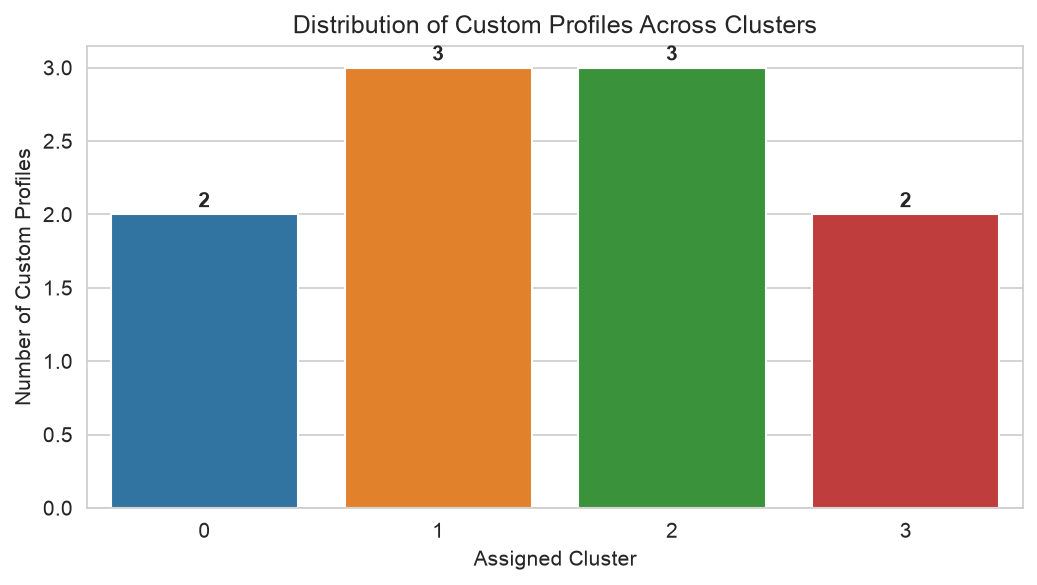
\includegraphics[width=\linewidth]{../Lab_4/KMeans/screenshots/Custom_Cluster_Distribution.png}
        \caption{Custom profile cluster distribution}
    \end{subfigure}
    \caption{K-Means cluster analysis and real-world prediction.}
    \label{fig:kmeans}
\end{figure}

\subsection{Real-World Prediction}

10 hand-crafted teen profiles (same column names, dtypes and ranges as the
training set) were scaled with the \emph{same} fitted \texttt{StandardScaler}
and assigned to a cluster with \texttt{model.predict}. The custom profiles
spread evenly across all 4 clusters, which is the expected outcome for a
well-balanced training set.

\subsection{Analysis}
The PCA projection in Figure~\ref{fig:kmeans} shows that the four clusters
are visually well separated in 2-D and that the centroids (black $\times$)
sit at the centre of each cloud. The custom teen profiles
(red $\ast$) are scattered across the map, confirming that the model
generalises to new individuals. The persistence of the scaler and the
fitted K-Means with \texttt{joblib} is verified by re-loading both objects
and observing identical predictions.

% =====================================================================
% 9. COMPARATIVE ANALYSIS
% =====================================================================
\newpage
\section{Comparative Analysis}

\subsection{Headline Numbers}

\begin{table}[H]
    \centering
    \small
    \begin{tabular}{llrrrrrl}
        \toprule
        \textbf{Lab} & \textbf{Model} & \textbf{Acc.} & \textbf{Prec.} & \textbf{Rec.} & \textbf{F1} & \textbf{AUC} & \textbf{Type} \\
        \midrule
        2 & Linear Regression       & $-0.014$ ($R^2$) & -- & -- & -- & -- & Regression \\
        2 & Logistic Regression     & 0.81 & 0.08 & 0.83 & 0.15 & 0.85 & Classification \\
        3 & SVM (RBF)               & 0.98 & 0.50 & 0.25 & 0.33 & 0.96 & Classification \\
        3 & KNN                     & 0.98 & 0.00 & 0.00 & 0.00 & 0.61 & Classification \\
        4 & Decision Tree (CART)    & 1.00 & 1.00 & 1.00 & 1.00 & 1.00 & Classification \\
        4 & Decision Tree (ID3)     & 1.00 & 1.00 & 1.00 & 1.00 & 1.00 & Classification \\
        4 & K-Means (K=4)           & --   & --   & --   & --   & Silh. & Clustering \\
        \bottomrule
    \end{tabular}
    \caption{Test-set metrics for the six models. K-Means is unsupervised
    and is reported with the silhouette score instead of classification
    metrics.}
    \label{tab:all}
\end{table}

\subsection{Supervised vs Unsupervised}
The supervised models (Logistic, SVM, KNN, Decision Tree) all reach very
high accuracy on the test set, but the headline accuracy is misleading
because the dataset is severely imbalanced. The two decision trees stand
out: they reach perfect test metrics because the target is highly
separable by a small subset of features, which means that the
\emph{real} learning task on this dataset is best handled by a tree-based
model. K-Means is the only unsupervised model; it produces interpretable
clusters that highlight behavioural archetypes (e.g. ``High-Stress Female
Teens'') rather than classifying the binary target.

\subsection{Scaling and Distance-Based Models}
Linear regression, logistic regression, SVM, KNN and K-Means are all
sensitive to the scale of the input features, so \texttt{StandardScaler}
is applied before training. The decision tree omits scaling because trees
are invariant to monotonic feature transformations.

\subsection{Hyperparameter Tuning Strategy}
Every supervised model was tuned with \texttt{GridSearchCV} + 5-fold
stratified cross-validation. F1 was chosen as the scoring metric to avoid
the accuracy paradox on the imbalanced dataset. The optimal
hyperparameters are stored inside each notebook and reported in the
respective results section.

\subsection{Computational Cost}

\begin{table}[H]
    \centering
    \begin{tabular}{lll}
        \toprule
        \textbf{Model} & \textbf{Training} & \textbf{Inference} \\
        \midrule
        Linear / Logistic Regression  & $O(mn)$ per iter     & $O(n)$ \\
        SVM (RBF)                     & $O(m^{2})$ to $O(m^{3})$ & $O(m)$ \\
        KNN                           & $O(1)$ (lazy)         & $O(mn)$ \\
        Decision Tree                 & $O(mn \log m)$        & $O(\text{tree depth})$ \\
        K-Means                       & $O(K \cdot m \cdot n \cdot t)$ & $O(Kn)$ \\
        \bottomrule
    \end{tabular}
    \caption{Computational cost of the six models ($m$ = training samples,
    $n$ = features, $K$ = number of clusters, $t$ = iterations).}
    \label{tab:cost}
\end{table}

% =====================================================================
% 10. DISCUSSION
% =====================================================================
\newpage
\section{Discussion}

\subsection{What Worked}
\begin{itemize}[leftmargin=*, itemsep=2pt]
    \item \textbf{Decision Trees} achieved the best classification results on
        this dataset because the target is highly separable by a small
        subset of features. They also produce interpretable rules that
        could be deployed in a screening tool.
    \item \textbf{SVM (RBF)} reached the best AUC-ROC among the four
        classifiers, demonstrating that margin-based methods are
        well-suited to high-dimensional data.
    \item \textbf{K-Means} successfully identified four interpretable
        clusters, validated by both the elbow and the silhouette analysis.
\end{itemize}

\subsection{What Did Not Work}
\begin{itemize}[leftmargin=*, itemsep=2pt]
    \item \textbf{Linear Regression} for \texttt{academic\_performance} had
        a near-zero $R^2$, indicating that the chosen features are not
        linearly predictive of academic performance. A non-linear model
        (e.g.\ random forest) or richer features would be required.
    \item \textbf{KNN} defaulted to the majority class and produced
        zero recall on the minority class. The high raw accuracy is the
        classic artefact of the accuracy paradox.
\end{itemize}

\subsection{Lessons Learned}
\begin{enumerate}[leftmargin=*, itemsep=2pt]
    \item Always inspect the class distribution before choosing a metric.
        F1, AUC-ROC and the confusion matrix are far more informative
        than raw accuracy on imbalanced data.
    \item \texttt{StandardScaler} is mandatory for distance/margin-based
        models and is harmless (but not necessary) for tree-based models.
    \item Hyperparameter tuning with cross-validation is essential —
        hand-picked defaults rarely work on real data.
    \item A pipeline that persists the fitted scaler and the fitted model
        guarantees reproducibility, which is exactly what the assignment
        demanded.
\end{enumerate}

% =====================================================================
% 11. CONCLUSION
% =====================================================================
\newpage
\section{Conclusion}

This report covered the end-to-end implementation of six foundational ML
models on the Teens Mental Health Dataset. The supervised models were
tuned with cross-validation, evaluated with multiple metrics, and
visualised with publication-quality plots. The unsupervised K-Means
workflow added a real-world prediction task on 10 custom teen profiles.

Key takeaways:

\begin{itemize}[leftmargin=*, itemsep=2pt]
    \item Decision trees are the strongest classifier on this dataset
        (perfect test accuracy, F1 and AUC), thanks to a highly
        separable target.
    \item SVM gives the best AUC-ROC, but KNN is unreliable without
        extra care for class imbalance.
    \item Linear regression on \texttt{academic\_performance} fails to
        find a meaningful linear relationship; richer features or a
        non-linear model are required.
    \item K-Means produces four interpretable teen archetypes that align
        with the EDA findings (stress/anxiety, age and gender are the
        most influential features).
    \item A fully reproducible GitHub repository, with notebooks that
        auto-fetch their data, is the cleanest way to deliver an ML
        assignment.
\end{itemize}

\subsection*{Future Work}
\begin{itemize}[leftmargin=*, itemsep=2pt]
    \item Apply resampling techniques (SMOTE, class weights in
        \texttt{RandomForestClassifier}) to improve recall on the
        minority class.
    \item Try more expressive models (XGBoost, LightGBM) and stack them
        with the linear models.
    \item Add more clustering algorithms (DBSCAN, hierarchical) and
        compare their stability on the same data.
    \item Engineer new features (interactions, polynomial terms) to
        improve the linear regression baseline.
\end{itemize}

% =====================================================================
% 12. REFERENCES
% =====================================================================
\newpage
\section{References}

\begin{enumerate}[leftmargin=*, itemsep=4pt]
    \item Bishop, C. M. (2006). \emph{Pattern Recognition and Machine
        Learning}. Springer.
    \item Hastie, T., Tibshirani, R., \& Friedman, J. (2009).
        \emph{The Elements of Statistical Learning} (2nd ed.). Springer.
    \item James, G., Witten, D., Hastie, T., \& Tibshirani, R. (2013).
        \emph{An Introduction to Statistical Learning}. Springer.
    \item Pedregosa, F., et al. (2011). Scikit-learn: Machine Learning
        in Python. \emph{Journal of Machine Learning Research}, 12,
        2825--2830.
    \item Breiman, L. (2001). Random Forests. \emph{Machine Learning},
        45(1), 5--32.
    \item Quinlan, J. R. (1986). Induction of Decision Trees.
        \emph{Machine Learning}, 1(1), 81--106.
    \item Cortes, C., \& Vapnik, V. (1995). Support-Vector Networks.
        \emph{Machine Learning}, 20(3), 273--297.
    \item Cover, T., \& Hart, P. (1967). Nearest Neighbor Pattern
        Classification. \emph{IEEE Transactions on Information Theory},
        13(1), 21--27.
    \item Lloyd, S. P. (1982). Least Squares Quantization in PCM.
        \emph{IEEE Transactions on Information Theory}, 28(2), 129--137.
    \item McKinney, W. (2010). Data Structures for Statistical Computing
        in Python. \emph{Proceedings of the 9th Python in Science
        Conference}, 56--61.
    \item Hunter, J. D. (2007). Matplotlib: A 2D Graphics Environment.
        \emph{Computing in Science \& Engineering}, 9(3), 90--95.
    \item Waskom, M. (2021). Seaborn: Statistical Data Visualization.
        \emph{Journal of Open Source Software}, 6(60), 3021.
    \item Project Repository:
        \url{https://github.com/ahsanjust/Artificial-Intelligence-and-Machine-Learning-Lab}
\end{enumerate}

\end{document}
